
\chapter{Metody kompensacji dyspersji}
\label{cha:comp_disp}
 
Istnieje wiele różnych metod kompensacji dyspersji w tej pracy szczegółowo opisane zostały wybrane trzy. Pierwsza polegająca na przygotowaniu sygnału, który sam skompensuje się do odpowiedniej postaci w trakcie propagacji. Druga bazująca na przybliżaniu krzywych dyspersji przy pomocy rozwinięcia w szereg Taylora, oraz trzecia polegająca na mapowaniu sygnału z dziedziny czasu na odległość 
 

\section{Cel kompensacji}
\label{sec:cel_komp}

\subsection{Zastosowanie fal Lamba w nieniszczacych testach}

Fale prowadzone akustyczne i ultradźwiękowe, w tym między innymi fale Lamba, są wykorzystywane na wiele sposobów między innymi do nieniszczących testów oraz oceny jakości obiektów. Stosowane są między innymi do diagnostyki uszkodzeń aktywnych lub pasywnych w monitorowaniu kondycji strukturalnej (SHM - Structural Health Monitoring). W niektórych przypakach fale te są wykorzystywane do uzyskania lokalnych informacji o próbce, której to informacji nie można uzyskać konwencjonalnymi technikami ultradźwiękowymi. Przykładem takiego zastosowania może być inspekcja spoiwa klejowego[2-Wilcox]. Jest to przykład aplikacji o krótkim zasięgu, ponieważ odległość propagacji fal kierowanych jest stosunkowo mała. Drugi obszar zastosowania kontroli fal prowadzonych jest przeznaczony do testowania dalekiego zasięgu. W tym przypadku odległość propagacji jest stosunkowo duża. Ich główną zaletą, sprawiającą, iż są one tak często wykorzystywane do diagnozy urządzeń jest to, że mogą być wzbudzane przez elementy uruchamiające znajdujące się na lub wewnątrz struktury w jednym punkcie konstrukcji i mogą się rozprzestrzeniać na duże odległości. Konwencjonalna kontrola ultradźwiękowa dużych struktur jest bardzo czasochłonna, ponieważ testom musi zostać poddany każdy punkt badanej struktury, która ma być monitorowana. Wykorzystanie fal Lamba jest więc potencjalnie bardzo atrakcyjnym rozwiązaniem tego problemu. Jeżeli przetwornik odbierający znajduje się w odległym punkcie struktury, odebrany sygnał zawiera informacje o całej przebytej ścieżce propagacji między przetwornikami nadawczym i odbiorczym. W związku z tym test monitoruje całą ściężkę, a nie pojedynczy punkt struktury. Pozwala to na znaczne zaoszczędzenie czasu badań. W przypadku prętów niejednokrotnie stosuje się techniki, w których nadajnik po wyemitowniu sygnału przełącza się w tryb odbiornika. Propagujący sygnał odbija się od końca pręta i wraca spowrotem, gdzie jest odbierany i może zostać poddany analizie. Takie podejście jest bardzo często stosowane, zwłaszcza w sytuacjach, w których dostęp do pręta możliwy jest tylko z jednej strony jak na przykład podczas badania kotw górniczych. Przykład ich położenia ilustruje rysunek \ref{fig:kotwy}
\begin{figure}[h]
\centering
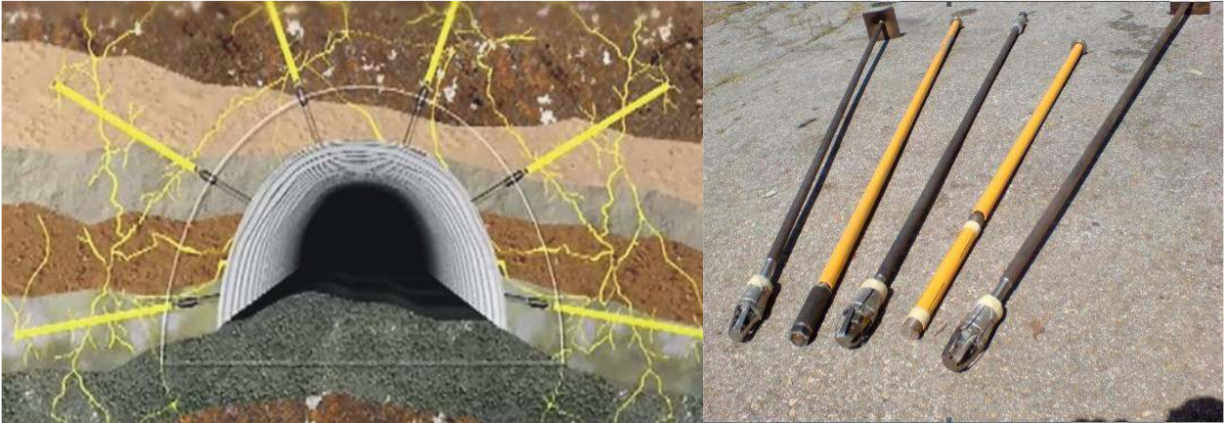
\includegraphics[width=14cm]{Zdjecia/4/kotwy}
\caption{Przykład zamontowania kotw górniczych, do których dostęp w przypadku testów jest tylko z jednej strony \ref{art:kotwy}}
\label{fig:kotwy}
\end{figure}

Nawet w najprostszych strukturach, takich jak swobodna płaska izotropowa płyta lub prosty stalowy pręt, może istnieć nieskończona liczba sterowanych trybów falowych. Co więcej, postaci te są generalnie dyspersyjne. Obydwa te fakty utrudniają praktyczne zastosowanie fal kierowanych. W praktyce testy kontroli dalekiego zasięgu są wykonywane w sposób zadowalający, gdy stosuje się tylko jedną lub czasami dwie postaci fal prowadzonych, a pozostałe są tłumione. Tradycyjnie osiąga się to za pomocą specjalnych przetworników. Dzięki starannej kontroli częstotliwości i liczby falowej wzbudzenia, możliwe jest generowanie wybranych postaci fali Lamba oraz tłumienie pozostałych. Kontrola zakresu częstotliwości może być osiągnięta przez użycie sygnału o pewnej szerokości pasma zamkniętego w oknie Hanninga lub Gaussa. Zakres liczby falowej może być ograniczony przez użycie starannie zaprojektowanych sond EMAT lub za pomocą piezoelektrycznego przetwornika. 

Powyższe metody mogą służyć do tłumienia sygnałów wywołanych przez niepożądane postaci fali, ale nie mogą zapobiec efektowi dyspersji, ponieważ zjawisko to występuje w falach kierowanych podczas ich propagacji w strukturze. Dyspersja sygnału powoduje, rozproszenie energii sygnału w czasie i przestrzeni w trakcie propagacji sygnału. W praktyce objawia się to wzrostem czasu trwania odbieranego sygnału w porównaniu do czasu trwania sygnału wejściowego. Rysunek \ref{fig:dyspersja} ilustruje przykład sygnału bez dyspersji oraz sygnału rozproszonego na skutek propagacji pewnej odległości. Łatwo zauważyć, że sygnał przed propagacją trwa zaledwie $0,0001 s$ natomiast po jego czas zwiększa się do około $0,0013s$ a zatem trwa ponad 10 razy dłużej.
\begin{figure}[h]
\centering
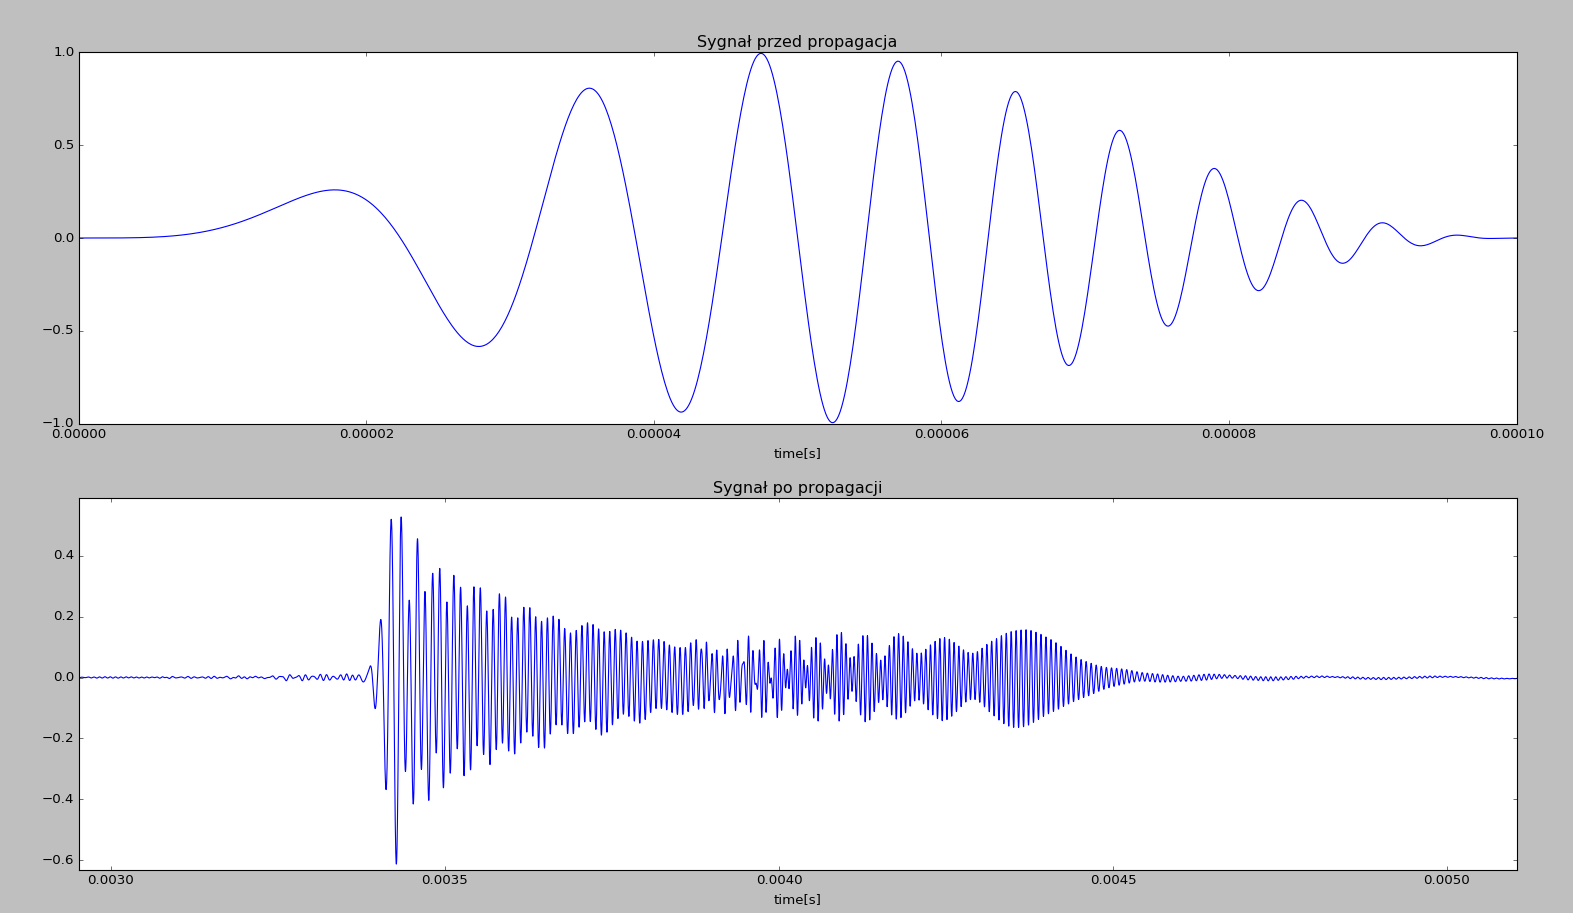
\includegraphics[width=14cm]{Zdjecia/4/dyspersja}
\caption{Przykład sygnału wejściowego, oraz sygnału rozproszonego}
\label{fig:dyspersja}
\end{figure}

 Zjawisko to pogarsza rozdzielczość i sprawia, że dane eksperymentalne są trudne do interpretacji z powodu nakładania się sygnałów. Używanie sygnałów wejściowych o określonej przepustowości może zmniejszyć problem dyspersji. Takie podejście koncentruje energię wejściową w ograniczonym zakresie częstotliwości, w którym jakiekolwiek zmiany prędkości pożądanego trybu fal kierowanych są małe. W praktyce oznacza to pracę w punktach na krzywych dyspersji dla konkretnego układu, w których prędkość grupowa jest stacjonarna lub prawie stacjonarna względem częstotliwości. Takie punkty zostały określone jako punkty "zerowej dyspersji" w\textcolor{red}{[1kasia]}, jest to określenie, które może wprowadzać w błąd, ponieważ niemożliwe jest skoncentrowanie całej energii sygnału wejściowego o skończonej długości na jednej częstotliwości. Zostało udowodnione \textcolor{red}{[2kasia]}, że istnieje optymalny sygnał wejściowy dla każdego punktu na krzywych dyspersji, który maksymalizuje rozdzielczość, jaką można uzyskać w tym punkcie. Jeśli jednak przyjmiemy, że przetwarzanie sygnału jest dozwolone przed wyświetlaniem informacji operatorowi, możliwe jest inne podejście do fal prowadzonych oraz ich roli w nieniszczących testach.

Należy również zaznaczyć, iż w praktyce rozproszone sygnały są zwykle uszkodzone z powodu szumów. Zachodzące na siebie i słabnące sygnały w porównaniu z szumem sprawiają, że dane z czujników są trudniejsze do interpretacji. W konsekwencji rodzielczość może ulec pogorszeniu. Dlatego zrodziła się ogromna potrzeba opracowania technik przetwarzania sygnałów w celu zwiększenia rozdzielczości czasowej i amplitudy SNR.

Z punktu widzenia systemów SHM, kompresja sygnału lub usuwanie dyspersji w dziedzinie czasu może być wygodnym i intuicyjnym sposobem na łatwiejszą interpretację sygnałów czujnika.

\subsection{Sygnał stosowany wy symulacji}
W ramach niniejszej pracy powstała aplikacja, pozwalająca użytkownikowi na podstawie podanych parametrów pręta wygenerować krzywe dyspersji opisujące dany obiekt. Aplikacja pozwala również na wygenerowanie sygnału testowego, symulację jego propagacji w zadanym pręcie, oraz kompensację otrzymanego sygnału wybranymi metodami. Sygnałem stosowanym do testów był sygnał chirp zmodyfikowany przypomocy okna Hanninga.
	Sygnał o nazwie chirp jest sygnałem sinusoidalnym, w którym faza jest funkcją czasu. \textcolor{red}{[3kasia]}. Sygnał o nazwie linear chirp to sygnał, w którym częstotliwość zmienia się w sposób liniowo zależny od czasu. Sygnał taki jest opisany wzorem:
	\begin{equation}
	s(t) = \sin(\phi (t))
	\end{equation}
	
	Gdzie $\phi (t)$ to funkcja fazy. Chwilową częstotliwość takiego sygnału jest związana funkcją fazy następującą zależnością:
	\begin{equation}
	f(t) = \frac{1}{2\pi}\frac{d(\phi (t))}{dt} \label{eq:f(t)_z_phi}
	\end{equation}
	
	Aby zatem wygenerować sygnał linear chirp o rządanych parametrach należy przyjąć, iż funkcja częstotliwości przybiera postać:
	\begin{equation}
	f(t) = f_0+\frac{B}{T}t \label{eq:f(t)_liniowo}
	\end{equation}
	
	Gdzie:
	
	$f_0$ - częstotliwość początkowa
	
	$B$ - szerokość pasma częstotliwości
	
	$T$ - czas trwania sygnału
	
	Łącząc równania (\ref{eq:f(t)_z_phi}) oraz (\ref{eq:f(t)_liniowo}) można funkcję fazy zapisać jako:
	\begin{equation}
	\phi (t) = 2\pi f_0t+\frac{\pi Bt^2}{T} \label{eq:phi(t)}
	\end{equation}
	A zatem pełen wzór opisujący sygnał linear chirp można zapisać jako:
	\begin{equation}
	s(t) = \sin(2\pi f_0t+\frac{\pi Bt^2}{T})
	\end{equation}
	
	Przykład funkcji częstotliwości oraz uzyskanego w ten sposób sygnału przedstawia rysunek \ref{fig:linear_chirp}
\begin{figure}[h]
\centering
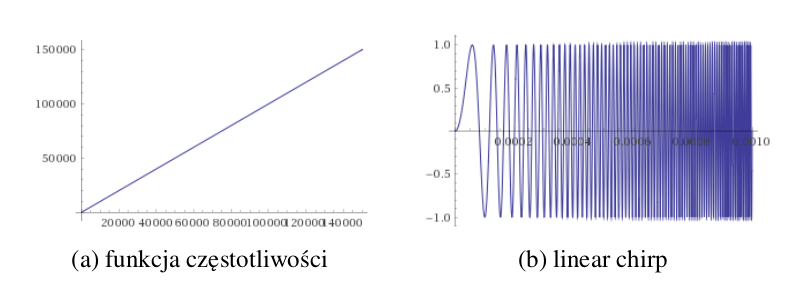
\includegraphics[width=14cm]{Zdjecia/4/linear_chirp}
\caption{Przykład sygnału linear chirp (b) oraz jego funkcji częstotliwości (a)}
\label{fig:linear_chirp}
\end{figure}

W prezentowanej pracy, sygnałem, który był poddawany symulacji był liniowy chirp dodatkowo pomnożony przez funkcję okna Hanninga daną wzorem:
\begin{equation}
w(n)=0,5(1-cos(\frac{2\pi n}{N-1})) \label{eq:okno_hanninga}
\end{equation}

Gdzie $N$ to całkowita liczba próbek. uzyskany w ten sposób sygnał został zaprezentowany na rysunku \ref{fig:test_chirp}
\begin{figure}[h]
\centering
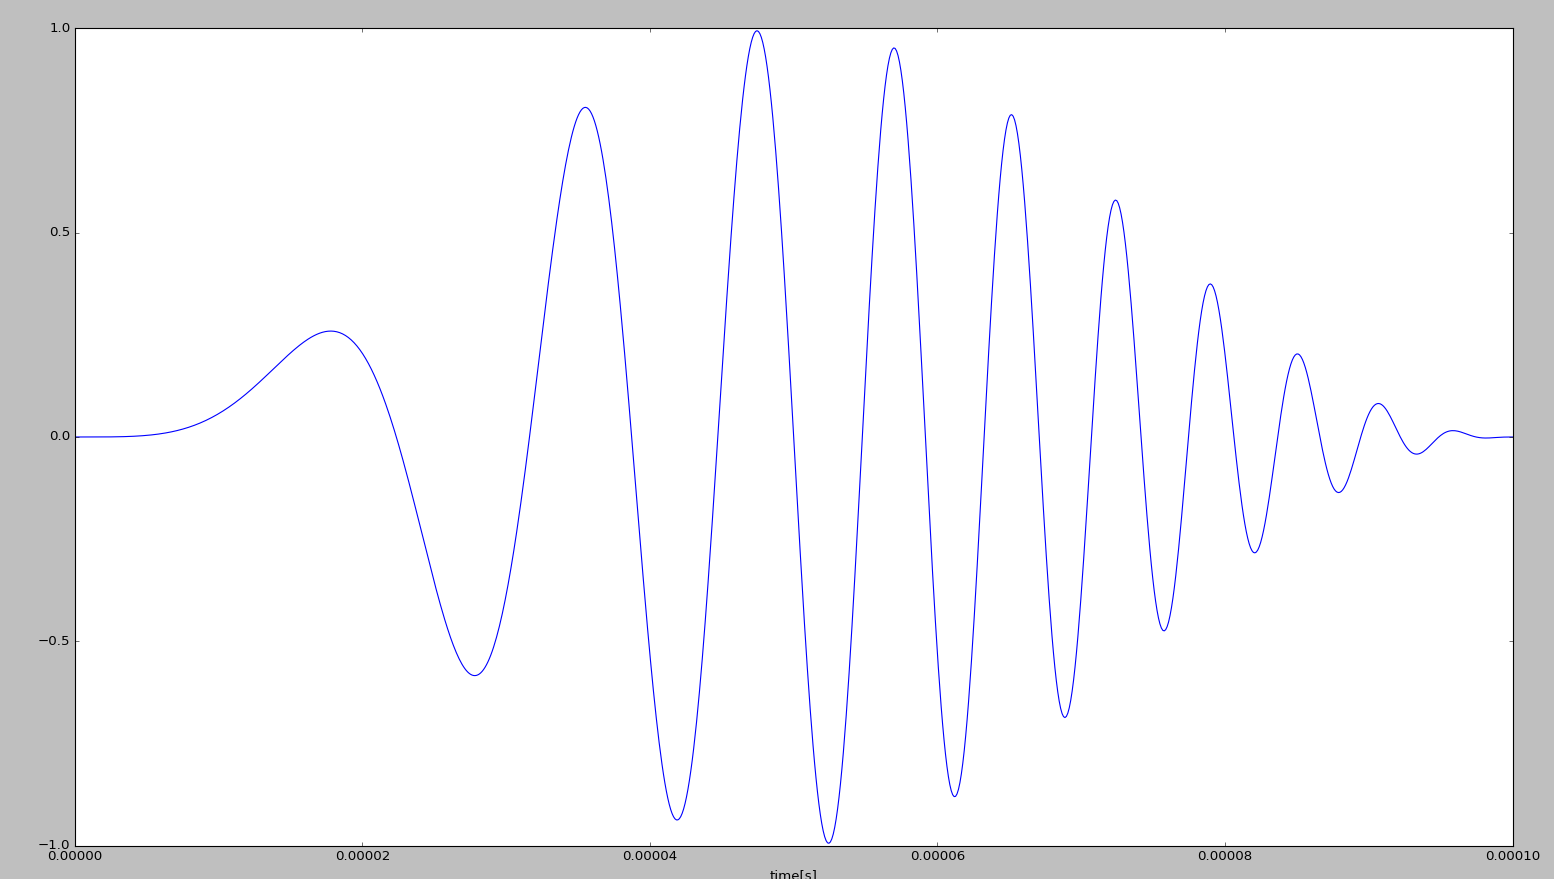
\includegraphics[width=14cm]{Zdjecia/4/test_chirp}
\caption{Linear chirp pomnożony przez funkcję okna Hanninga}
\label{fig:test_chirp}
\end{figure}

W aplikacji zaimplementowany został algorytm generujący opisany wyżej sygnał o następujących parametrach:

\begin{itemize}
\item czas trwania sygnału - 0.0001s
\item częstotliwość minimalna - 0Hz
\item częstotliwość maksymalna - 100kHz
\end{itemize}

Całość stworzona jest w oparciu o koncepcję otwartego koduco daje użytkownikowi możliwość pisania własnych funkcji, generujących dowolne sygnały a następnie ich bezproblemową symulcję w stworzonej aplikacji.

\section{Agregacja krzywych dyspersji uzyskanych z zaimplementowanego solvera}
\label{sec:agregacja}

\subsection{Cel agregacji}
Podstawą opracowania każdej z przedstawionych w tej pracy metod kompensacji jest znajomość krzywych dyspersji badanego obiektu, jakim jest stalowy pręt. Stanowią one pewnego rodzaju funkcję przejścia sygnału pomiędzy jednym punktem w czasie i przestrzeni a dowolnym innym punktem. Ich znajomość stanowi więc klucz do skompensowania efektu dyspersji. W stworzonej aplikacji, dzięki zastosowaniu odpowiednich algorytmów oraz na podstawie odpowiednich zadanych parametrów badanego obiektu, otrzymywane są poszukiwane krzywe dyspersji. Jednak dane są one w postaci chmury punktów zapisywanych w odpowiednich plikach. Aby funkcje te nadawały się do użycia należy każdy z wygenerowanych punktów przypisać do odpowiadającej krzywej. W ten sposób uzyskane zostaną funkcje, z których każda opisywać będzie zachowanie innej postaci fali prowadzonej. Przykładowe wygenerowane krzywe dyspersji przed agregacją przedstawia rysunek 2.21

\subsection{Algorytm agregacji}
 Krzywe dyspersji wyrażają zależność liczby falowej od częstości kątowej. Jako wynik w aplikacji otrzymujemy pojedynczy wektor zawierający kolejne wartości liczby falowej oraz zestaw odpowiadających danej liczbie częstości kątowych. Pierwszym krokiem w agregacji tak zapisanych danych jest zapisanie wszystkich danych w postaci chmury punktów o dwóch współrzędnych $A=(\omega , k)$ oraz posortowanie ich rosnąco wartościami $\omega$. Liczba wygenerowanych krzywych odpowiada ilości punktów posiadających tę samą współrzędną k. Ponieważ są to wartości własne równania (2.44) to dla każdej wartości k jest ich tyle samo. Każda krzywa składa się z dokładnie takiej liczby punktów jaka jest długość wektora k. Kolejnym krokiem jest przyporządkwanie pierwszych dwóch punktów do każdej z krzywych. Mając punkty uporządkowane względem $\omega$ wystarczy wybrać te o najmniejszej wartości k. Każdy z nich odpowiada kolejnemu trybowi fali. Punkty przydzielone do właściwego trybu zostają usunięte ze zbioru punktów do przydzielenia. Analogicznie postępujemy w przypadku drugiej grupy punktów. Wybieramy te o najniższej wartości k i przypisujemy do poszczególnych trybów. Agregacja kolejnych punktów musi przebiegać według innego schematu, ponieważ krzywe się wzajemnie przecinają i segregacja względem częstotliwości nie przyniesie zadowalających rezultatów. Przyjmując, że dla dowolnego modu, ostatni zagregowany punkt ma współrzędne $P_l = (\omega _l,k_l)$ z chmury punktów wybieramy zbiór potencjalnych punktów spełniających następujące warunki:
 \begin{enumerate}
 \item Wartość k potencjalnych punktów musi wynosić $k=k_p=v_k[l+1]$
 
 Gdzie $k_p$ oznacza wartość k potencjalnych punktów, $v_k$ oznacza posortowany rosnąco wektor wartości k, a $l+1$ to indeks wartości z wektora $v_k$ o jeden większy niż indeks ostatnio zagregowanego do danego trybu punktu
 \item Wartość $\omega$ potencjalnych punktów musi znajdować się w pewnym, ograniczonym otoczeniu wartości $\omega _l$
 
 Ze zbioru potencjalnych punktów, które spełniają wyżej wymienione warunki należy następnie wybrać ten, który w najepszy sposób będzie pasował do powstałego już fragmentu krzywej dyspersji. W celu wybrania najlepszego punktu obliczony zostaje kąt pomiędzy wektorami $\overrightarrow{v_1} = \overrightarrow{P_{l-1}P_l}$ oraz $\overrightarrow{v_2} = \overrightarrow{P_lP_{p_i}}$, gdzie $P_{p_i}$ oznacza i-ty potencjalny punkt ze zbioru. Sformułowanie najlepiej pasujący punkt oznacza, iż kąt pomiędzy rozważanymi wektorami, obliczany ze wzoru:
 \begin{equation}
 \alpha = \arccos\frac{\overrightarrow{v_1} \circ \overrightarrow{v_2}}{|\overrightarrow{v_1}|\cdot|\overrightarrow{v_2}|}
\end{equation}  
ma wartość najbliższą zeru. Usuwając zagregowane już punkty ze zbioru punktów do przydzielenia oraz postępując w sposób analogiczny do przedstawionego schematu, wszystkie punkty ze zbioru zostają przydzielone odpowiedniej krzywej. Wyniki agregacji zostały przedstawione na rysunku \ref{fig:krzywe_po_agregacji}
 
\begin{figure}[h]
\centering
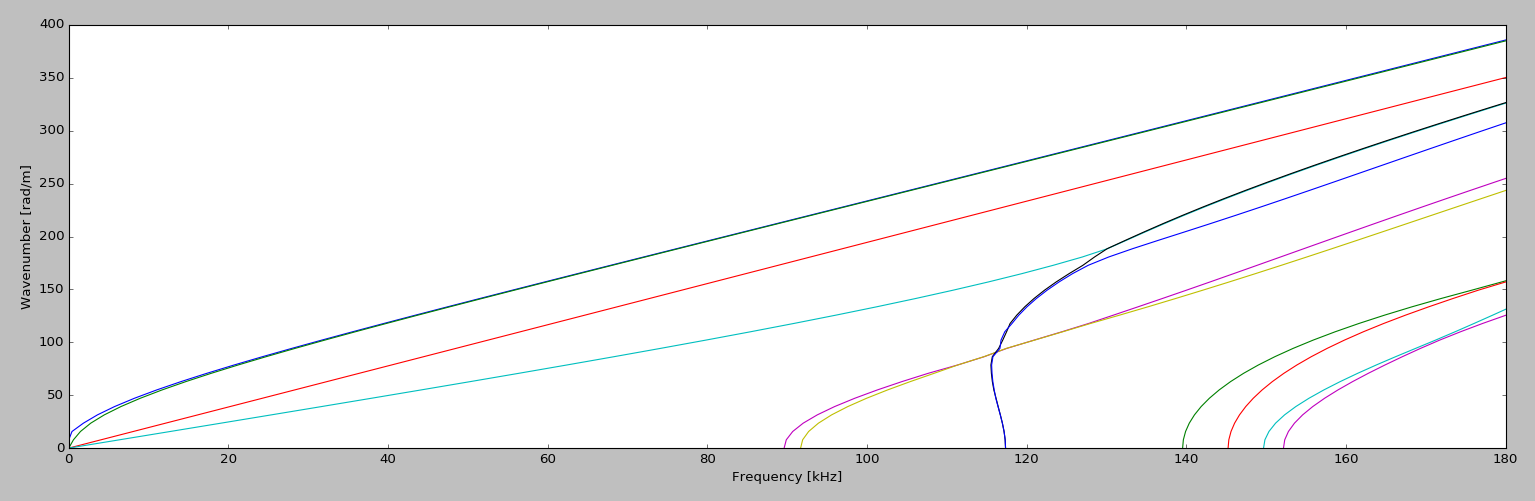
\includegraphics[width=13cm]{Zdjecia/4/zagregowane_krzywe}
\caption{Krzywe dyspersji po agregacji}
\label{fig:krzywe_po_agregacji}
\end{figure}
\end{enumerate}  

Jak łatwo zauważyć opisany algorytm w sposób efektywny agreguje chmurę punktów do odpowiednich krzywych. Uporządkowoane w ten sposób punkty zostały wykorzystane do opracowania trzech metod kompensacji, opisanych w kolejnych sekcjach tego rozdziału.





\section{Metoda odwracania sygnału w czasie}
\label{sec:metoda_tr}

Metoda omawiana w tej sekcji polega na wygenerowaniu sygnału który po przepropagowaniu pewnej odległości sam się skompensuje. Technika kompensacji dyspersji poprzez wygenerowanie sygnału odwróconego w czasie została zaprezentowana w artykule \cite{kasia4}

\subsection{Podstawy teoretyczne}
Podstawową ideą prezentowanej w tej części pracy techniki kompensacji dyspersji jest wytworzenie sygnału, który poprzez nałożenie składowych częstotliwości w czasie propagacji skompensuje się, tworząc oczekiwany sygnał w pozycji pomiarowej. W przypadku w którym do obiektu wprowadzony zostanie zwykły sygnał sinusoidalny o liniowo zmieniającej się częstotliwości (linear-chirp) zostanie wzbudzone przynajmniej kilka trybów fali prowadzonej. Każdy tryb w każdej z częstotliwości może poruszać się z różną prędkością fazową i grupową. Ze względu na dyspersję sygnał wraz z propagacją będzie stawał się coraz dłuższy a jego amplituda będzie spadać, ponieważ ulegnie on rozproszeniu.  Składowe częstotliwości sygnału odpowiadające najwyższym prędkością grupowym będą znajdować się z przodu, natomiast wolniejsze komponenty będą znajdowały się z tyłu. Podstawa przedstawianej metody polega na założeniu, że tak otrzymany sygnał jesteśmy w stanie odwrócić w czasie, tak aby komponenty o mniejszej prędkości znalazły się z przodu sygnału a komponenty o większej prędkości znalazły się z tyłu. Wzbudzenie obiektu tak przygotowanym sygnałem da w odpowiedzi sygnał skompensowany tej samej postaci co pierwotne wzbudzenie. Skuteczność metody można wykazać analitycznie. Przyjijmy, że sygnał zastosowany do wzbudzenia pręta zostanie zastosowany w punkcie $x = 0$ i będzie to sygnał $f(t)$. Sygnał wzbudzający w dziedzinie częstotliwości możemy zapisać jako:
\begin{equation}
[F(\omega)_{x=0}]=\int\limits_{-\infty}^{\infty}f(t)e^{-i\omega t}dt \label{eq:F(omega)_x=0}
\end{equation}
Jeśli przez nasz obiekt propaguje jedna postać fali to w punkcie $x=L$ można tę funkcję zapisać jako:

\begin{equation}
[F(\omega)_{x=L}]=\int\limits_{-\infty}^{\infty}f(t)e^{-i(\omega t - kL}dt \label{eq:F(omega)_x=L}
\end{equation}

gdzie liczba falowa k jest funkcją częstotliwości $\omega$  , która jest opisana za pomocą krzywej dyspersji dla danego trybu fali. Równania (\ref{eq:F(omega)_x=0}) oraz (\ref{eq:F(omega)_x=L}) można powiązać funkcją przejścia $H(\omega)$ co można zapisać jako:
\begin{equation}
H(\omega) = \frac{[F(\omega)]_{x=L}}{[F(\omega)]_{x=0}} \label{eq:h(omega)}
\end{equation}

Zakładając, że chcemy uzyskać sygnał $g(t)$, którego transformata Fouriera to $G(\omega)$ przy ($x = L$) wtedy wymagany sygnał wejściowy ($x = 0$) $Y(\omega)$:
\begin{equation}
Y(\omega) = \frac{G(\omega)}{H(\omega)} = G(\omega)[H(\omega)]^{-1} \label{eq:Y(omega)}
\end{equation}
Sygnał w dziedzinie czasu y(t) jaki musi zostać wprowadzony do badanego pręta w punkcie $x=0$ aby uzyskać odebrany sygnał $g(t)$ w punkcie $x=L$ można uzyskać z odwrotnej transformaty Fouriera, co pokazuje równanie (\ref{eq:Y(omega)}):
\begin{equation}
y(t) = \frac{1}{2\pi}\int\limits_{-\infty}^{\infty}\frac{G(\omega)}{H(\omega)}e^{i\omega t}d\omega \label{eq:y(t)}
\end{equation}

W prostym przypadku gdy analizujemy pojedynczą postać fali prowadzonej:
\begin{equation}
[H(\omega)]^{-1} = e^{-ikL} = e^{-i\omega L/c}
\end{equation}
\begin{equation}
y(t) = \frac{1}{2\pi}\int\limits_{-\infty}^{\infty}G(\omega)e^{-i\omega (L/c - t)}d\omega
\end{equation}

Przyjmując, że sygnał w domenie czas $g(t)$ jest aplikowany w punkcie $x = 0$ sygnał $y^*(t)$ w punkcie x = L można zapisać jako:
\begin{equation}
y^*(t) = \frac{1}{2\pi}\int\limits_{-\infty}^{\infty}G(\omega)e^{-i\omega (L/c + t)}d\omega
\end{equation}

Technika kompensacji w tym przypadku polega na odebraniu sygnału $y^*(t)$ w przedziale czasowym $t\in [0,T]$ w którym cała paczka falowa zostanie odebrana przez odbiornik. Następnie sygnał zostaje odwrócony w czasie. Otrzymany w ten sposób sygnał może być zaaplikowany do badanego pręta. W trakcie propagacji zostanie on skompensowany do fali o kształcie takim jak kształt sygnału $g(t)$

\subsection{Implementacja numeryczna}
W ramach niniejszej pracy, omawiana metoda została zaimplementowana do aplikacji. Podstawa jej działania opiera się na znajomości krzywych dyspersji. Pierwszym etapem jest wygenerowanie sygnału, jaki chce się uzyskać w wyniku kompensacji. Następnie dzięki zaimplementowanym metodom należy uzyskać przewidywany kształt sygnału po przepropagowaniu zadanej odległości oraz odrócenie go w czasie. Sygnał otrzymany z tak przygotowanego sygnału wejściowego powinien skompensować się na zadanej odległości. Rysunek \ref{fig:kolejne_etapy_TR} przedstawia opisane kroki na przykładzie sygnału linear chirp.
\begin{figure}[h]
\centering
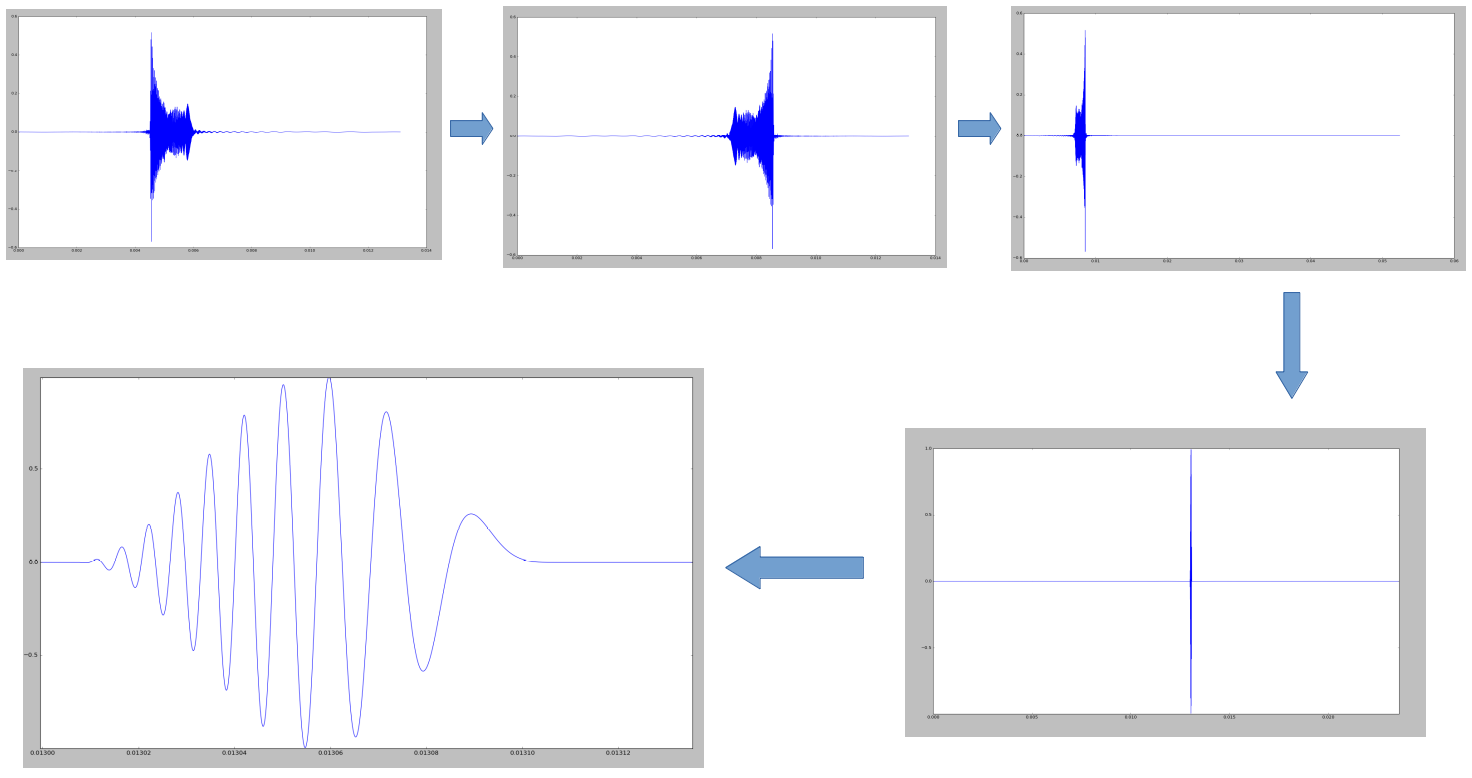
\includegraphics[width=14cm]{Zdjecia/4/algorytm_komp_tr}
\caption{Algorytm kompensacji odwracania czasu}
\label{fig:kolejne_etapy_TR}
\end{figure}

W zaprezentowanym przykładzie odwrócony w czasie sygnał został dodatkowo wypełniony zerami. Zabieg ten został zastosowany, ponieważ całość została przeprowadzona w ramach symulacji i wypełnienie sygnału było konieczne do przeprowadzenia prawidłowej symulacji propagacji. Przedstawiana metoda pozwala zatem wygenerować sygnał kompensujący się na zadanej odległości do fali o oczekiwanym kształcie. Pozwala na propagowanie zarówno pojedynczego trybu jaki nałożonych wielu postaci fali prowadzonej. Jednak aby móc stosować tę motodę konieczna jest znajomość długości ścieżki propagacji sygnału. Jeżeli ściażka propagacji ulegnie zmianie, konieczne jest wygenerowanie nowego sygnału adekwatnego do aktualnego badanego obiektu. W przypadku w którym podczas propagacji następowałyby dodatkowe odbicia, na przykład w sytuacji, w której fala propagujące przez dwa pręty złączone ze sobą, część energii zostanie odbita od punktu złączenia a część przepropaguje przez drugi pręt i odbije się na końcu. Stworzenie sygnału kompensującego się w takiej sytuacji byłoby bardziej skomplikowane i nie zostało opisane w tej pracy. Rysunek \ref{fig:rozne_odl} prezentuje przykład fali przygotowanej do kompensacji po 4 metrach propagacji, który przepropagował kolejno 1,2,4 i 5 metrów.

\begin{figure}[h]
\centering
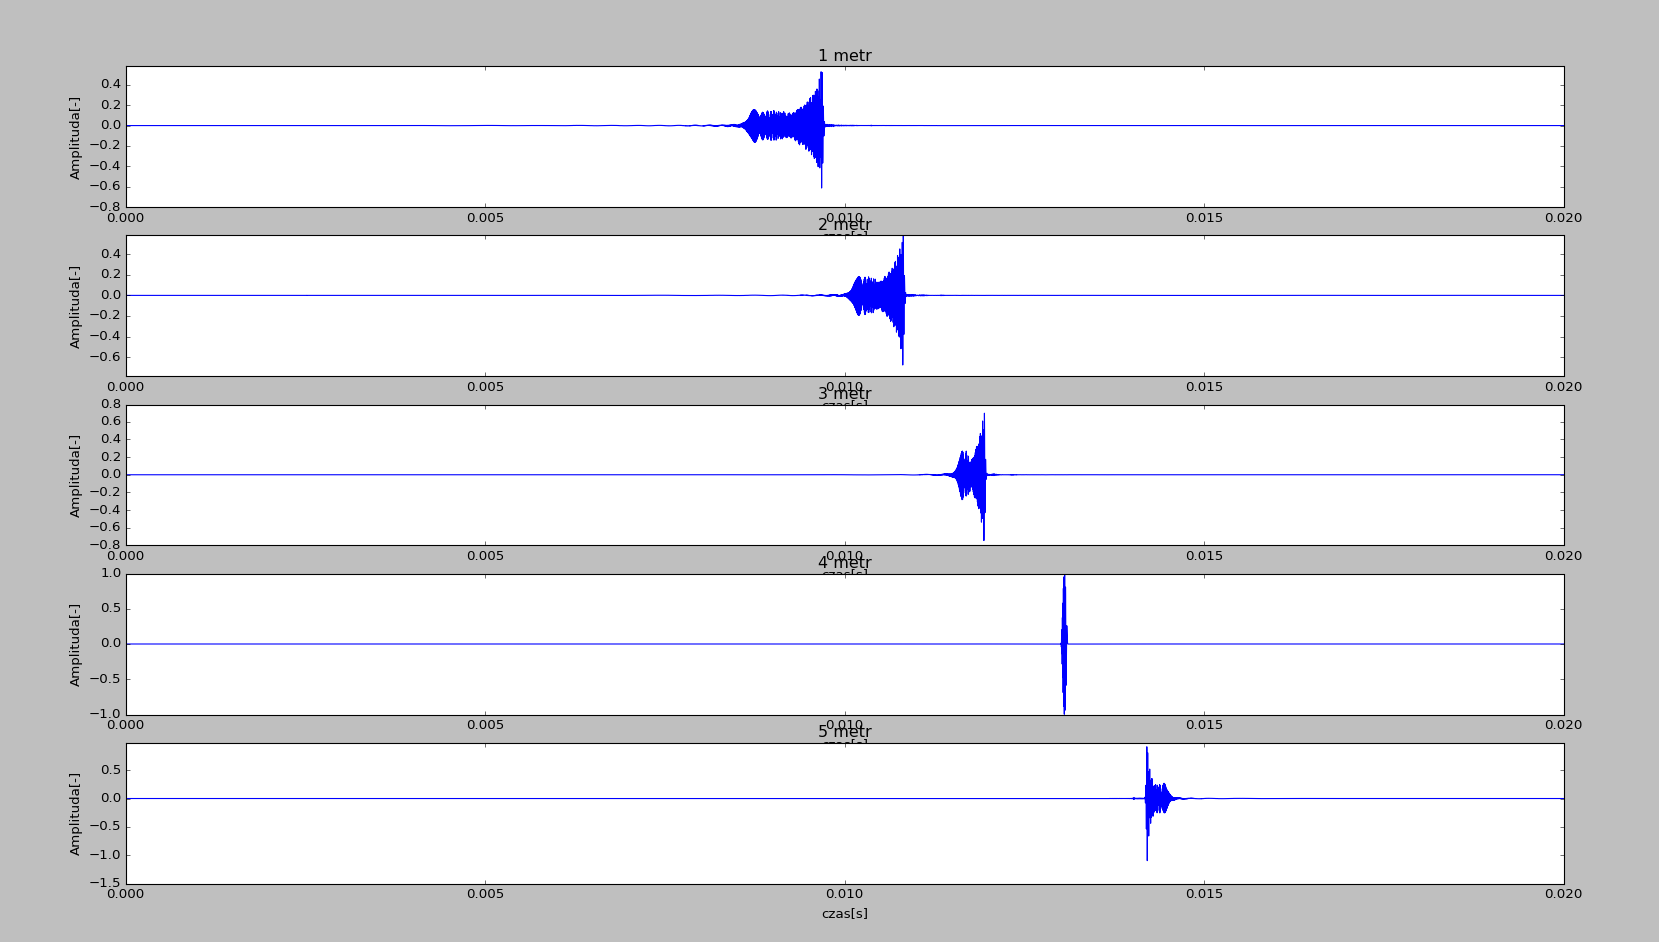
\includegraphics[width=14cm]{Zdjecia/4/porownanie_roznych_odleglosci_time_reversal}
\caption{Sygnał przygotowany do kompensacji po 4 metrach propagacji przedstawiony kolejno po 1, 2, 4 i 5 metrach propagacji}
\label{fig:rozne_odl}
\end{figure}

Jak łatwo zauważyć wprowadzony sygnał kompensuje się tylko i wyłącznie po przepropagowaniu założonej odległości. wraz z oddalaniem się od punktu, w którm przewidziany był odbiornik efekt dyspersji się nasila. Tak więc zarówno przed jak i za założonym punktem odbioru odebrany sygnał byłby rozproszony. Metoda ta może służyć do przeprowadzania nieniszczących testów obiektów o znanej charakterystyce przejścia. W sytuacji w której w strukturze nie będzie żadnych uszkodzeń otrzymywany sygnał będzie skompensowany. Natomiast gdy pojawią się uszkodzenia, nieciągłości w strukturze spowodują odbicie fali i skrócenie ścieżki propagacji co da informację o uszkodzeniach. 

\subsection{Wybrane wyniki z symulacji}
Rysunek \ref{fig:sygnal we} przedstawia sygnał przekazany do funkcji, jako ten, do którego sygnał ma się skompensować po przepropagowaniu zadanej odległości
\begin{figure}[h]
\centering
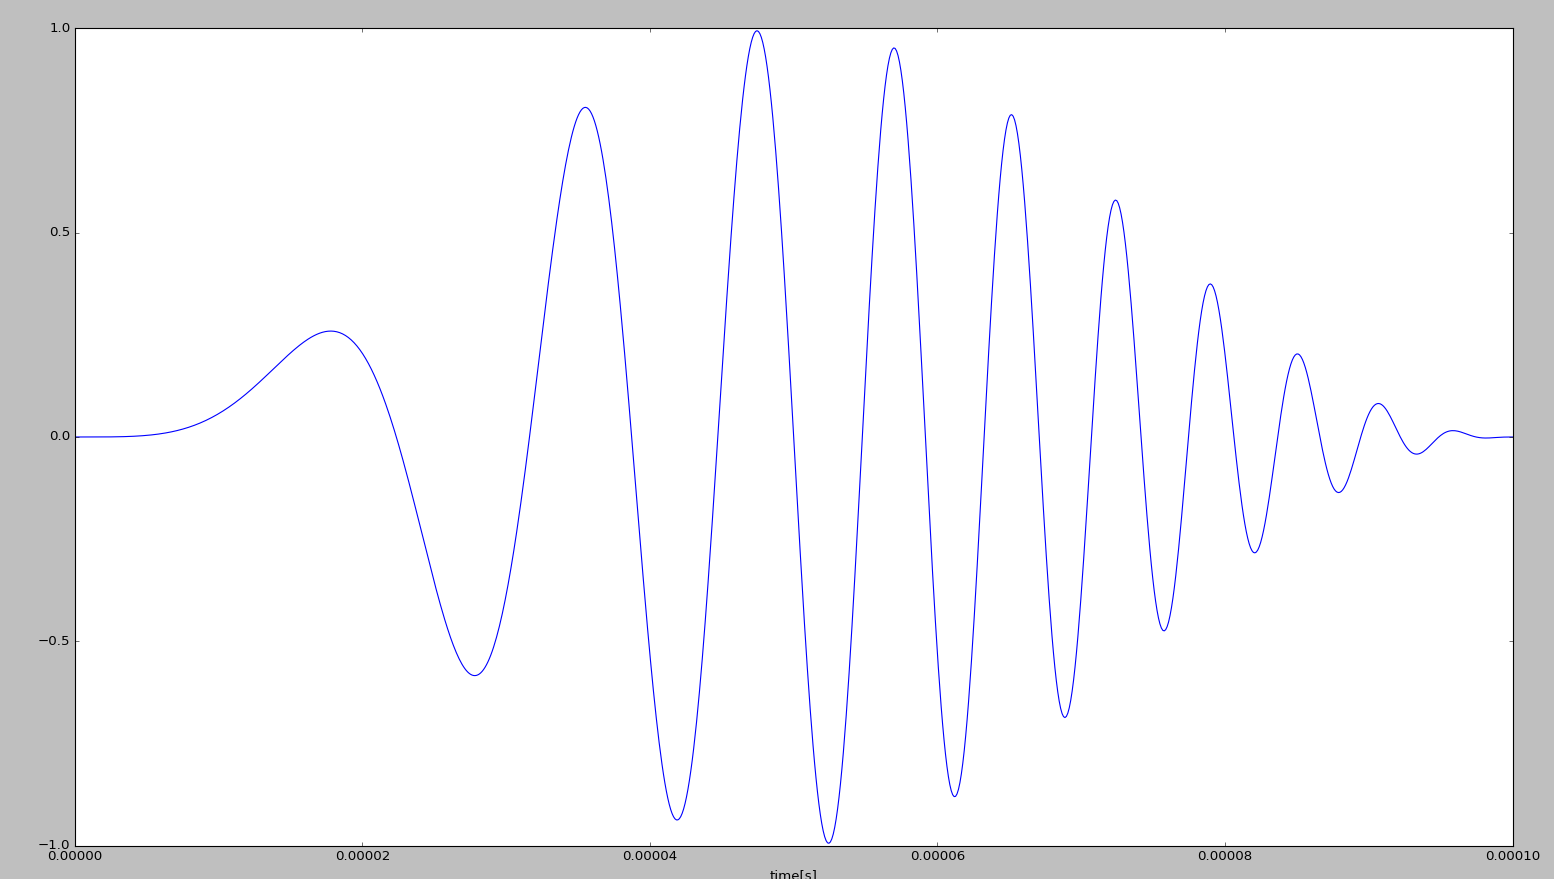
\includegraphics[width=14cm]{Zdjecia/4/test_chirp}
\caption{Algorytm kompensacji odwracania czasu}
\label{fig:sygnal we}
\end{figure}
Wygenerowany przez aplikację sygnał jest różny dla różnych zadanych odległości. Obrazuje to rysunek \ref{fig:rozne_odl} na którym przedstawiono sygnały mające się skompensować odpowiednio po 1, 2, 3, 4 metrach, gdy propagują pierwsze cztery postaci fali prowadzonej. 
\begin{figure}[h]
\centering
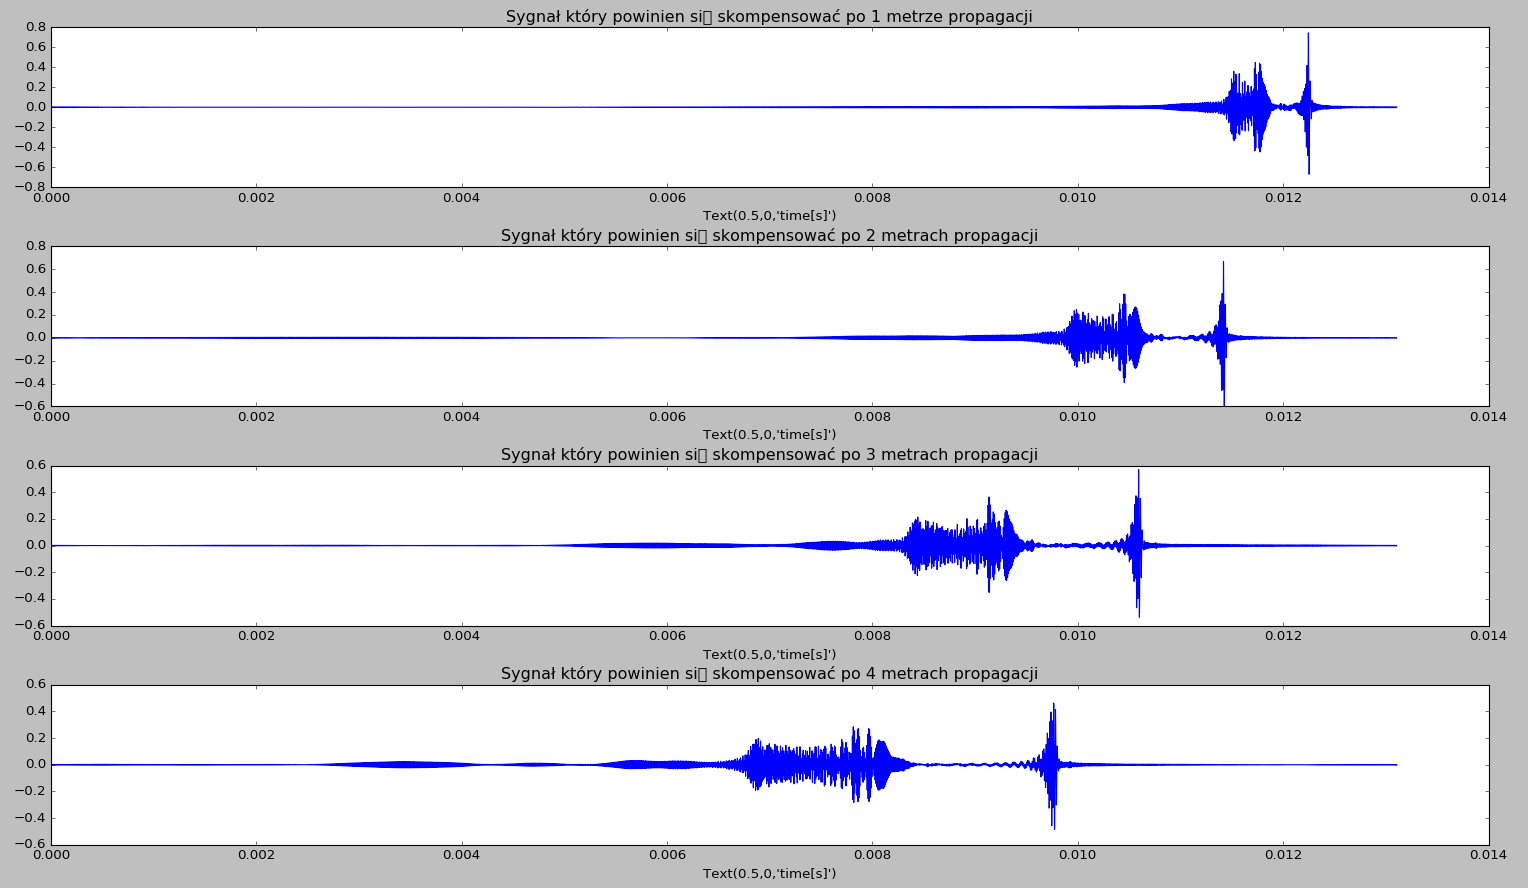
\includegraphics[width=14cm]{Zdjecia/4/tr_przykl}
\caption{Sygnał przygotowany do kompensacji po odpowiedno 1,2,3 oraz 4 metrach}
\label{fig:rozne_odl}
\end{figure}
Sygnał jest też różny dla różnej ilości propagujących trybów, rysunek \ref{fig:rozne_tryby}. Jak łatwo zauważyć, im większa ilość propagujących postaci tym bardziej widoczne staje się zjawisko dyspersji i tym dłuższy staje się przepropagowany sygnał.
\begin{figure}[h]
\centering
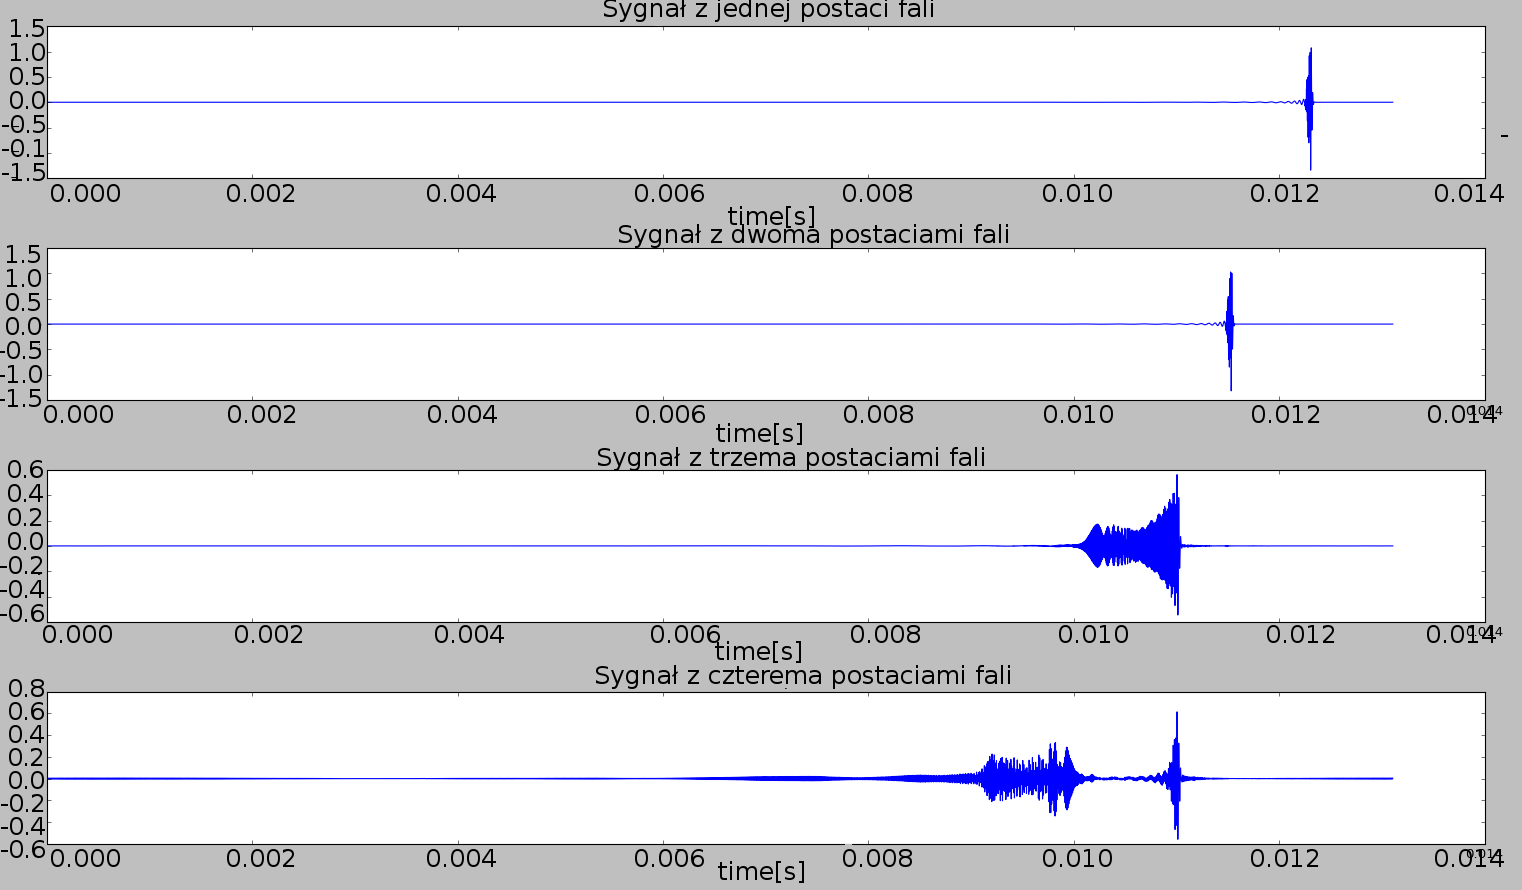
\includegraphics[width=14cm]{Zdjecia/4/TR-rozna_ilosc_modow}
\caption{Sygnał przygotowany do kompensacji po 2,5 metra propagacji zawierający kolejno 1,2,3 oraz 4 postaci fali prowadzonej}
\label{fig:rozne_tryby}
\end{figure}
Tak wygenerowane sygnały zostały przetestowane przez propagację w symulacji. Rysunek \ref{fig:100} ilustruje jak ważna jest znajomość długości ścieżki propagacji. Jeśli sygnał przebędzie zbyt krótką lub zbyt długą drogę to odebrany sygnał nie będzie skompensowany.
\begin{figure}[h]
\centering
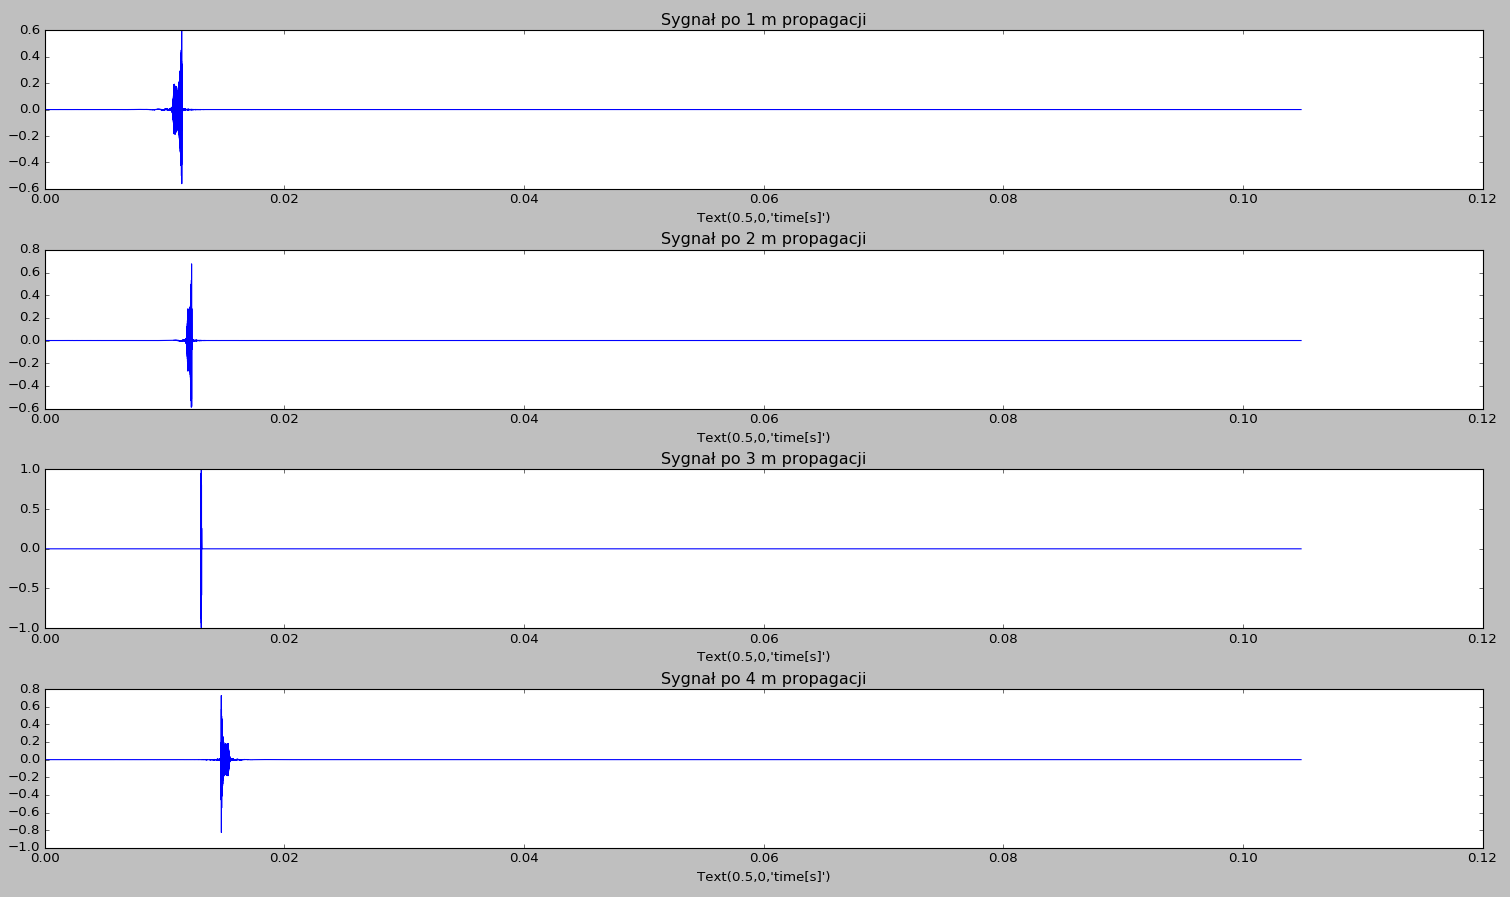
\includegraphics[width=14cm]{Zdjecia/4/obrazek100}
\caption{Sygnał przygotowany do kompensacji po 3 metrach propagacji przepropagowany kolejno o 1,2,3 i 5 metrów}
\label{fig:100}
\end{figure}
Rysunek \ref{fig:skompensowane_TR} ilustruje wyniki symulacji propagacji na odpowiednie odległości sygnałów przedstawinych na rysunku 4.9
\begin{figure}[h]
\centering
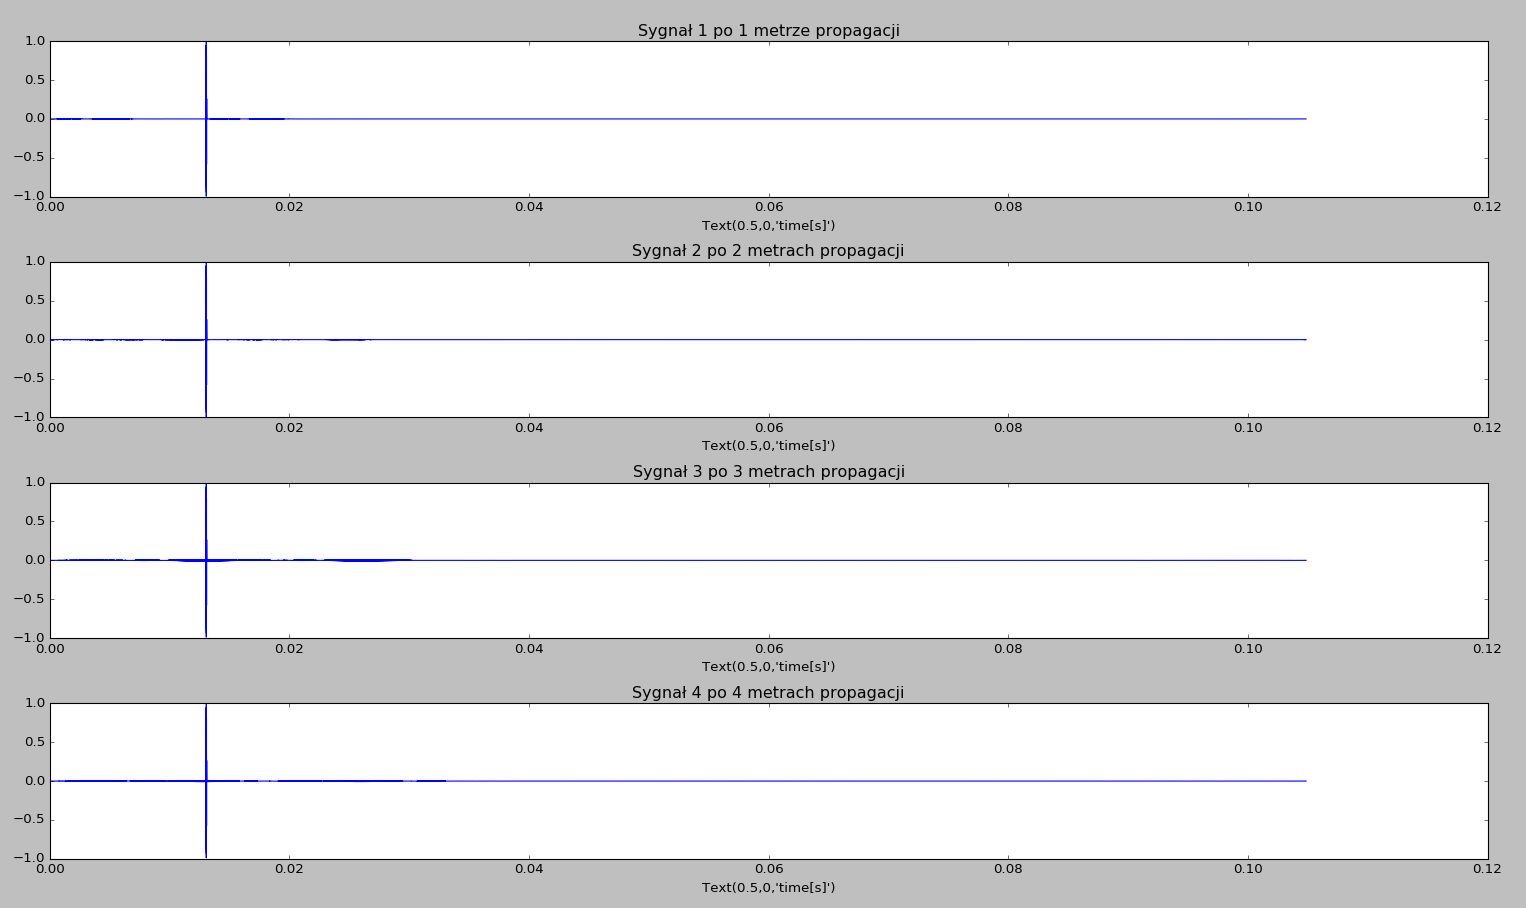
\includegraphics[width=14cm]{Zdjecia/4/skompensowane_TR}
\caption{Sygnały  z rysunu 4.9 po przepropagowaniu odpowiednich odległości}
\label{fig:skompensowane_TR}
\end{figure}

Rysunek \ref{fig:tr_rozna_il_postaci_skomp} ilustruje wyniki  symulacji propagacji sygnałów przedstawionych na rysunku 4.10. Łatwo zauważyć, że wyniki symulacji dają bardzo dobre rezultaty. 
\begin{figure}[h]
\centering
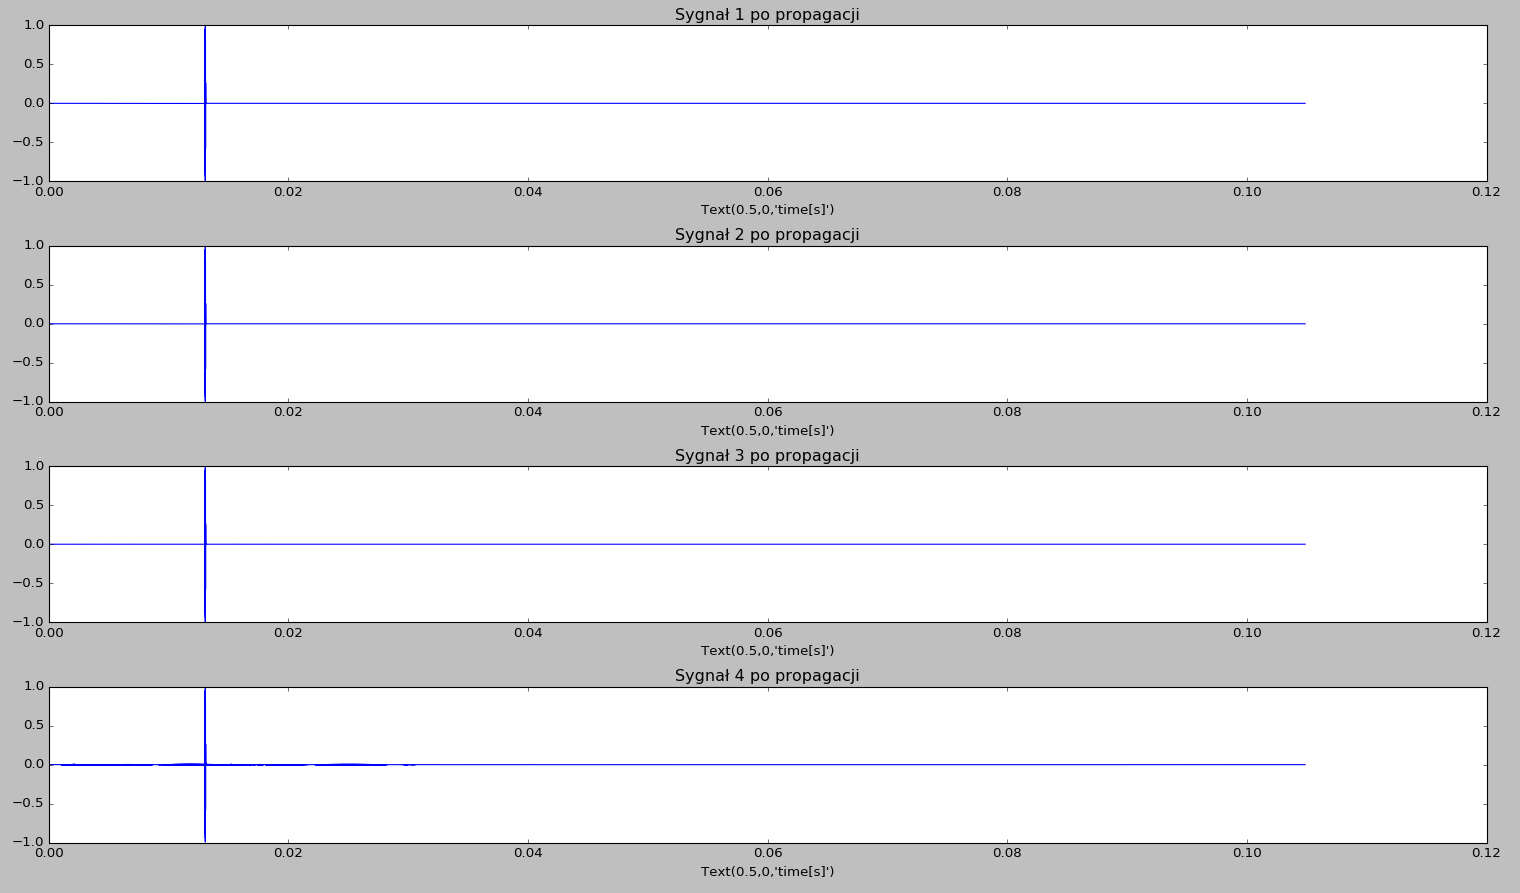
\includegraphics[width=14cm]{Zdjecia/4/tr_rozna_il_postaci_skomp}
\caption{Sygnały  z rysunu 4.10 po przepropagowaniu odpowiedniej odległości}
\label{fig:tr_rozna_il_postaci_skomp}
\end{figure} 

Rysunek \ref{fig:porownanie} przedstawia porównanie wyniku symulacji sygnału linear chirp po propagacji dwóch metrów w pręcie w którym propagowały trzy pierwsze tryby fali prowadzonej (kolor niebieski) oraz sygnału wygenerowanego w aplikacji, przygotowanego do kompensacji po dwóch metrach. Łatwo zauważyć, że przedstawiana metoda pozwala znacząco skrócić czas trwania odbieranego sygnału. Sygnał bez kompensacji trwa 6e-4s natomiast z 1e-4 czyli dokładnie tyle ile żądany sygnał. A zatem można stwierdzić iż kompensacja została skutecznie przeprowadzona. Kolejny rysunek przedstawia porównanie sygnału założonego na wejściu, jako jako postać do której powinien on zostać skompensowany, oraz sygnału faktycznie otrzymanego po symulacji propagacji. Czas trwania oraz obwiednia sygnału zgadzają się z założeniami, jednak widać iż otrzymany sygnał jest sygnałem odwróconym w czasie w stosunku do założonego sygnału. Wynik nie jest zatem idealnym odwzorowaniem założeń, niemniej jednak otrzymany sygnał został maksymalnie skompensowany. W otrzymanym sygnale nie ma również widocznych szumów, pogarszających czytelność otrzymanego wyniku. Oczywistym jest fakt, iż w przypadku rzeczywistym szumy z pewnością by występowały. Idealne matematyczne odwzorowanie padanego obiektu nie jest możliwe, lecz mimo to metoda powinna dawać dobre rezultaty.

\begin{figure}[h]
\centering
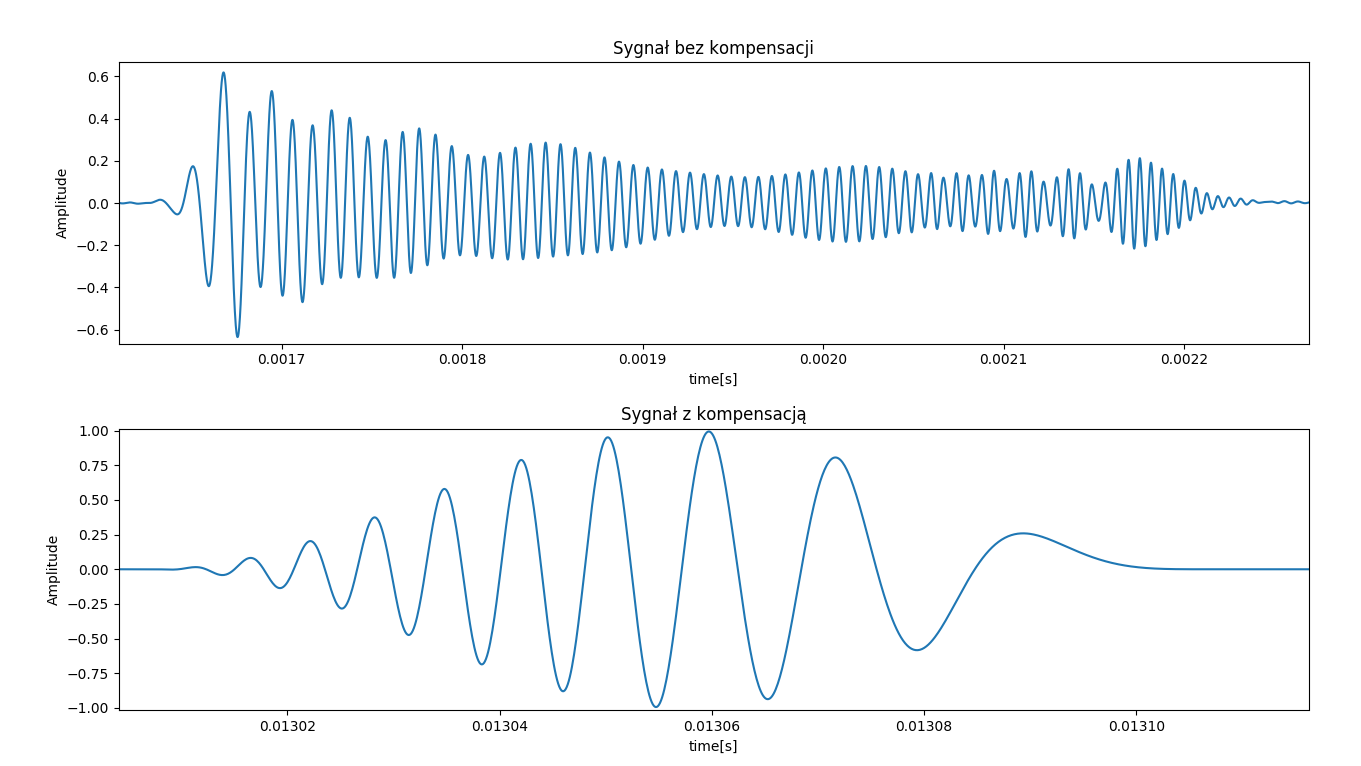
\includegraphics[width=14cm]{Zdjecia/4/tr_porownanie}
\caption{Porównanie sygnału bez kompensacji(górny) oraz z kompensacją (dolny)}
\label{fig:porownanie}
\end{figure} 

\begin{figure}[h]
\centering
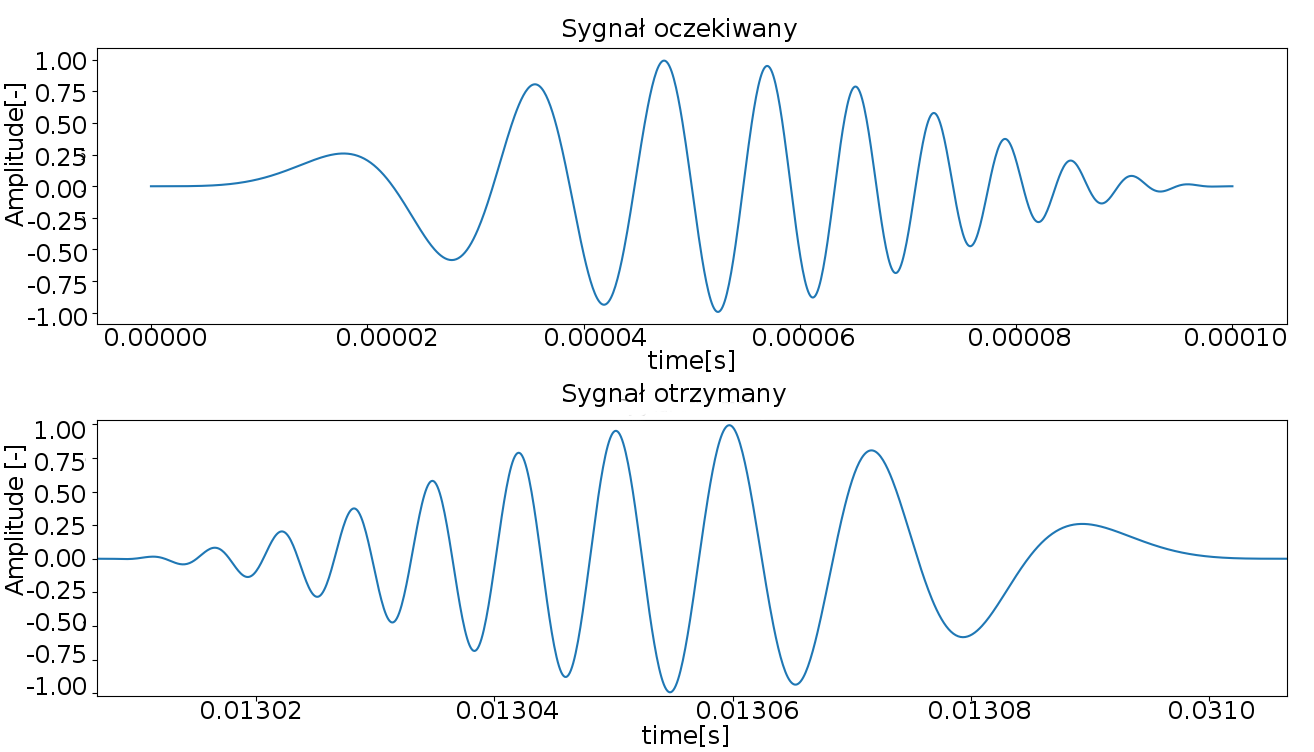
\includegraphics[width=14cm]{Zdjecia/4/tr_porownanie2}
\caption{Porównanie sygnału oczekiwanego(górny) otrzymanego (dolny)}
\label{fig:porownanie2}
\end{figure} 


\section{Metoda mapowania liniowego przy pomocy rozwinięcia w szereg Taylora}
\label{sec:Taylor}
Prezentowana w poniższej sekcji metoda kompensacji dyspersji została przedstawiona w artykule []\textcolor{red}{referenacja do yuanliu}
\subsection{Podstawy teoretyczne}
Po wzbudzeniu badanego pręta odpowiednim sygnałem wejściowym, możliwe jest aby przełączył się on w tryb obioru sygnału i nasłuchiwał nadejścia odpowiedzi układu. W takim wypadku odpowiedź jaką uzyskamy będzie sumą odpowiedzi ze wszystkich odbić, od końca pręta oraz ewentualnych łączeń lub uszkodzeń.  Proponowana w tym rozdziale metoda opiera sie na założeniu, że w badanym obiekce propaguje jedna wybrana postać drgań. Jej celem jest kompensacja powstałej dyspersji, tak aby sygnały z różnych punktów odbicia nie nachodziły na siebie i była możliwa ich interpretacja w celu ustalenia ilości punktów odbicia oraz oszacowania ich odegłości od miejsca wzbudzenia na podstawie znajomości prędkości grupowej fali. Przy tak sformułowanych założeniach, sygnał otrzymany w odbiorniku można przedstawić wzorem:
\begin{equation}
g(t) = \sum\limits_{n=1}{N}f_n(r_n,t)=\frac{1}{2\pi}\int _{-\infty}^{\infty}F(\omega)\sum\limits_{n=1}^{N}(A_n(\omega)e^{-ikr_n})e^{i\omega t} d\omega \label{eq:g(t)_taylor}
\end{equation}
Gdzie:

$N$ - całkowita liczba ścieżek propagacji sygnału (liczba punktów odbicia)

$r_n$ - długość n-tej ścieżki propagacji

$A_n$ - współczynnik odbicia n-tego punktu odbicia.

Widmo częstotliwości takiego sygnału $G(\omega)$  możemy obliczyć przy pomocy transformaty Fouriera i zapisać wzorem:
\begin{equation}
G(\omega) = F(\omega)\sum\limits_{n=1}^{N}(A_n(\omega)e^{-ikr_n} \label{eq:G(omega)_taylor}
\end{equation}

Jak wiadomo, dyspersja zależy od kształtu krzywej dyspersji, $k = K(\omega)$. Jeśli więc $K(\omega)$ jest funkcją kwadratową lub wyższego rzędu względem $\omega$, to $G(\omega)$ reprezentuje widmo częstotliwości rozproszonych pakietów fal. Jeśli natomiast zależność $K(\omega)$ byłoby funkcją liniową, zjawisko dyspersji nie występowałoby, a $G(\omega)$ reprezentowałoby widmo częstotliwości sygnału, który nie uległ dyspersji. 
Wybraną krzywą dyspersji można przybliżyć przy pomocy rozwinięcia w szereg Taylora:
\begin{equation}
k = K(\omega) - k_0+k_1(\omega - \omega _0) + k_2(\omega - \omega _0^2)+... \label{eq:szereg_k}
\end{equation}

Gdzie:

$k_0 = \frac{\omega _0}{c_p}$

$k_1 = \frac{dk}{d\omega}|_{\omega = \omega_0}$

$k_2 = \frac{1}{2}\frac{d^2k}{d\omega ^2}|_{\omega = \omega _0}$

$c_p$ - prędkość fazowa

Wynika z tego, iż dyspersję sygnału można usunąć usuwając jej nieliniowy składnik, poprzez zastąpienie oryginalnej zależności $K(\omega)$ liniowym przybliżeniem tej funkcji. Zastosowanie takiego zabiegu sprawi, iż sygnał w dziedzinie czasu będzie postrzegany jako skompensowany do postaci niedyspersyjnej, a prędkość grupowa obliczona z liniowego przybliżenia krzywej dyspersji może zostać wykorzystana do określenia długości ścieżek propagacji wynikających z kolejnych odbić. 

W szczególnym przypadku, w którym mamy do czynienia z pojedyńczą ścieżką propagacji ($N=1$) i odległość między nadajnikiem a punktem odbicia jest znana, można usunąć dyspersję poprzez wyeliminowanie wyrażenia kwadratowego w $K(\omega)$. Matematycznie można to zrobić przy pomocy wzoru:
\begin{equation}
 \widetilde{G}(\omega)=(F(\omega)A_1(\omega)e^{-ikr_1})e^{ik_2(\omega -\omega _0)^2r_1}
\end{equation}

Gdzie $\widetilde{G}(\omega)$ jest zmodyfikowanym widmem częstotliwości, a $r_1$ jest odległością między nadajnikiem i odbiornikiem. Sygnał skompensowany w dziedzinie czasu można natychmiast uzyskać poprzez odwrotną transformatę Fouriera. Ponieważ jednak zazwyczaj długość ścieżki propagacji sygnału nie jest znana, a sygnał może składać się z wielu odbić, między innymi od uszkodzeń ($N>1$) usuwanie dyspersji przy pomocy powyższego wzoru byłoby niepraktyczne. 

Rysunek \ref{fig:krzywa_taylorem} obrazuje przykład krzywej dyspersji, trybu $A_0$, płyty aluminiowej o grubości 3,175 mm. Linia ciągła pokazuje zależności $K(\omega)$ uzyskaną metodami komputerowymi, natomiast linia przerywana kropkowana wskazuje z rozwinięcie szeregu Taylora pierwszego rzędu, a linia przerywana rozszerzenie szeregu Taylora drugiego rzędu w odniesieniu do centralnej częsości kątowej ($\omega _0 = 2\pi *50 kHz$)

\begin{figure}[h]
\centering
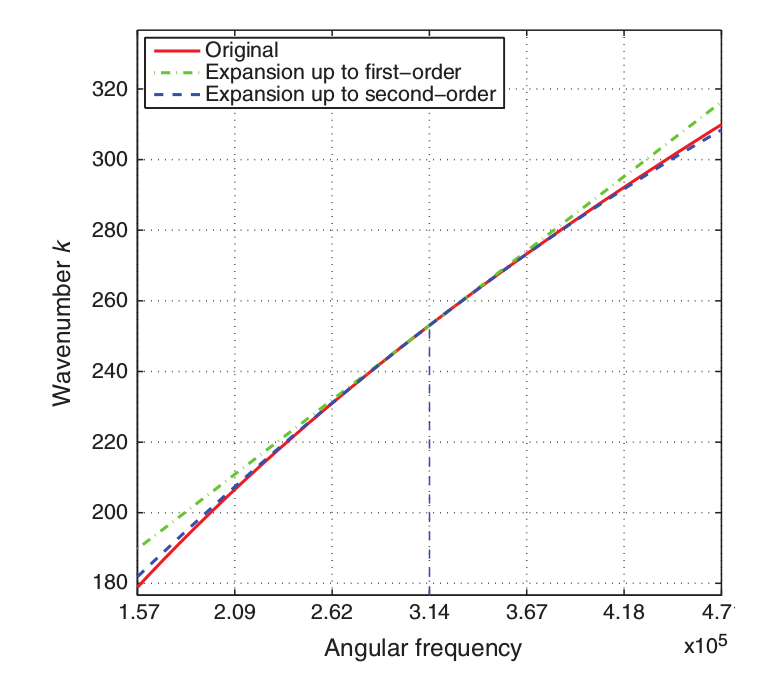
\includegraphics[width=14cm]{Zdjecia/4/buba}
\caption{Przykładowe porównanie oryginalnej krzywej oraz jej przybliżeń przy pomocy rozwinięcia w szereg Taylora}
\label{fig:krzywa_taylorem}
\end{figure}

Łatwo zauważyć, że po pierwsze, rozszerzenie drugiego rzędu daje bardzo dobrze przybliżenie pierwotnego kształtu krzywej, po drugie, $K(\omega)$ jest monotoniczną funkcją $\omega$ w otoczeniu $\omega _0$. 

Równanie \ref{eq:G(omega)_taylor} można zapisać w postacji złożenia funkcji:
\begin{equation}
G(\omega) = G(k)\circ K(\omega)
\end{equation}

Gdzie $\circ$ jest operatorem składania funkcji. $G(k)$ jest niejawną funkcją k z równania \ref{eq:G(omega)_taylor}. Zamieniając $K(\omega)$ na $K_{lin}(\omega)$ będące aproksymacją $K(\omega)$ pierwszego rzędu w punkcie $\omega _0$, gdzie $\omega _0$ oznacza częstotliwość o najwyższej energii, można wyprowadzić zmodyfikowane widmo częstotliwości:
\begin{equation}
\widetilde{G}(\omega) = G(k)\circ K_{lin}(\omega)
\end{equation}

Ponieważ $G(\omega)$ jest znane oraz znana jest analizowana krzywa dyspersji, znane jest również $G(k)$, obliczając przybliżenie liniowe $K_{lin}(\omega)$ można w prosty psosób obliczyć $\widetilde{G}(\omega)$, poprzez interpolację odpowiednich wartości. Opisana metoda może być określana mianem mapowania liniowego. W jej efekcie uzyskane zostaje nowe widmo częstotliwości $\widetilde{G}(\omega)$. Po mapowaniu widmo amplitudy pozostaje bez zmian, natomiast widmo fazy stopniowo odbiega od pierwotnego w miarę oddalania się od wybranej, środkowej częstotliwości, co dobrze ilustruje rysynek \ref{fig:widma}

\begin{figure}[h]
\centering
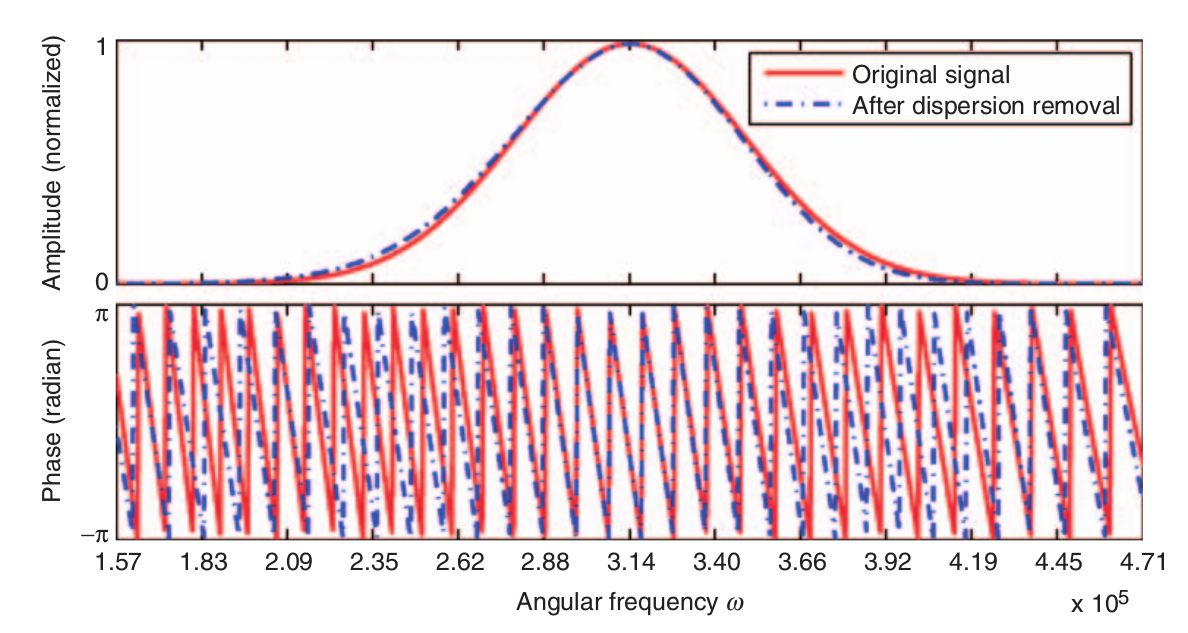
\includegraphics[width=14cm]{Zdjecia/4/widma}
\caption{Przykładowe porównanie oryginalnych charakterystyk oraz ich przybliżeń przy pomocy rozwinięcia w szereg Taylora}
\label{fig:widma}
\end{figure}

Należy zaznaczyć, iż stosowanie omawianej metody jest możliwe tylko w sytuacji, gdy $K(\omega)$ jest funkcją monotoniczną

\subsection{Implementacja numeryczna}
Implementacja prezentowanej metody opiera się głównie na znajomości krzywej dyspersji, której propagację bierzemy pod uwagę. Pierwszym krokiem, jest wygenerowanie odpowiedniego sygnału testowego. Mając właściwy sygnał można przystąpić do właściwego procesu kompensacji. W pierwszej kolejności analizowane jest widmo amplitudowe otrzymanego sygnału. Na jego podstawie uzyskiwana jest informacja o częstotliwości z największą energią. Zostaje ona wybrana na częstotliwość w której nastąpi przybliżenie liniowe. Po wybraniu $\omega _0$ odnajdywane jest na krzywej dyspersji odpowiednia wartość liczby falowej. Korzystając z zależności opisujących wartości $k_0$ i $k_1$ wyliczone zostaje liniowe przybliżenie badanej krzywej. Uzyskane w aplikacji wyniki przedstawia rysunek \ref{fig:krzywa_moja}. Linia niebieska prezentuje oryginalną krzywą dyspersji, natomiast linia zielona przdstawia jej przybliżenie uzyskane w aplikacji przy użyciu rozwinięcia w szereg Taylora.

\begin{figure}[h]
\centering
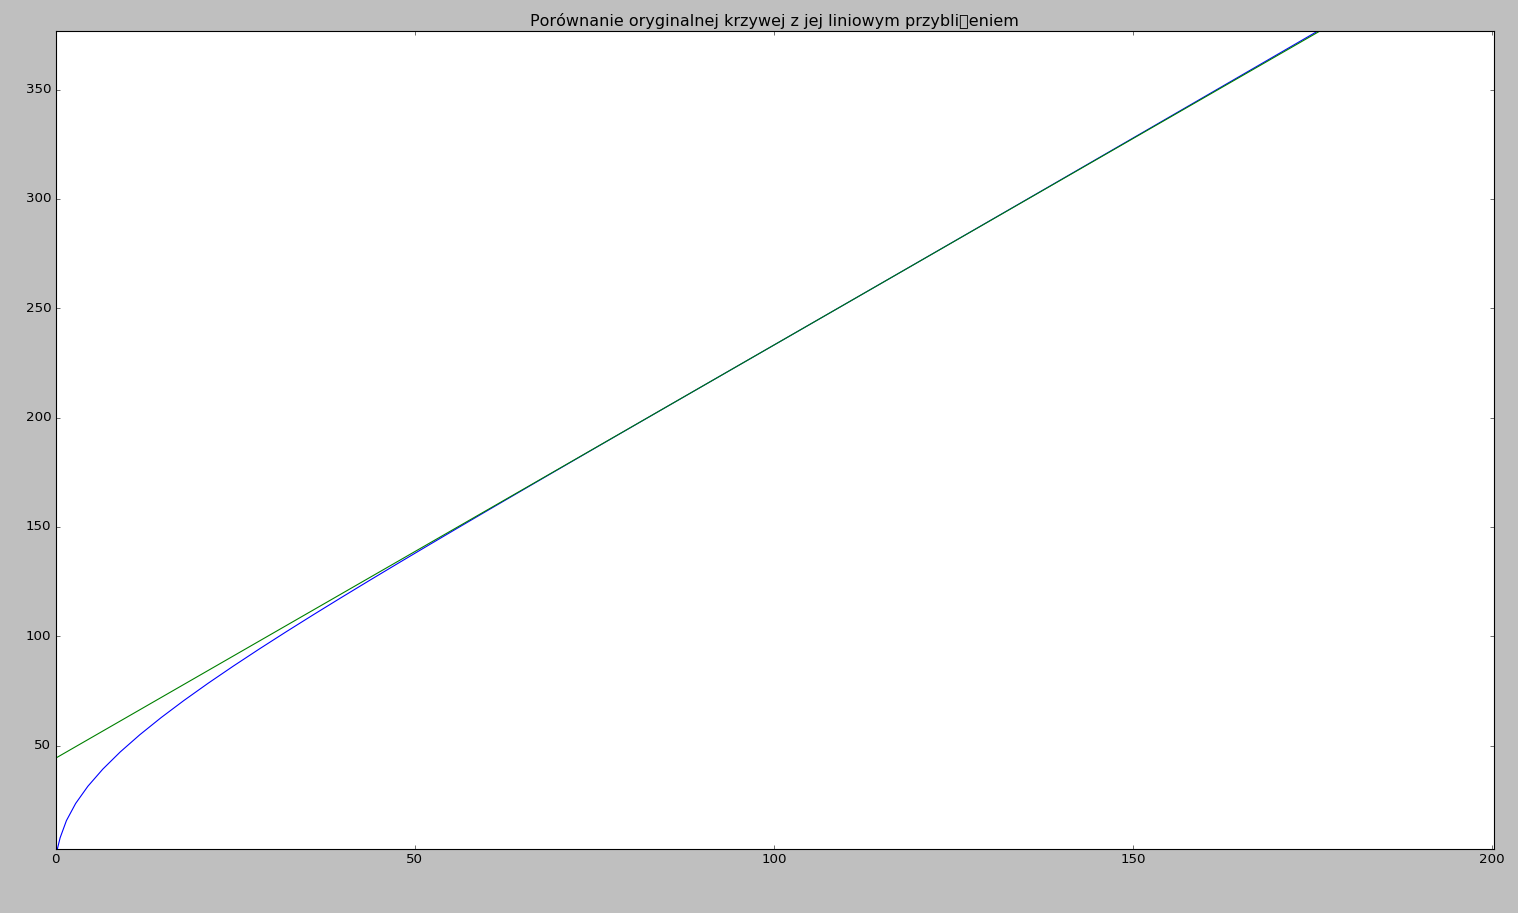
\includegraphics[width=14cm]{Zdjecia/4/krzywa_moja}
\caption{Przykładowe porównanie oryginalnej krzywej oraz jej przybliżeń przy pomocy rozwinięcia w szereg Taylora}
\label{fig:krzywa_moja}
\end{figure}

Kolejnym krokiem implementowanego algorytmu, jest wyliczenie G(k) na podstawie otrzymanego widma sygnału $G(\omega)$ na podstawie krzywej dyspersji. Następnie ponowne wyznaczenie zależności w dziedzinie częstotliwości, tym razem jednak używając przybliżenia liniowego zamiast oryginalnej krzywej dyspersji. Omawiany algorytm doskonale ilustruje rysunek \ref{fig:algo_Taylora}

\begin{figure}[h]
\centering
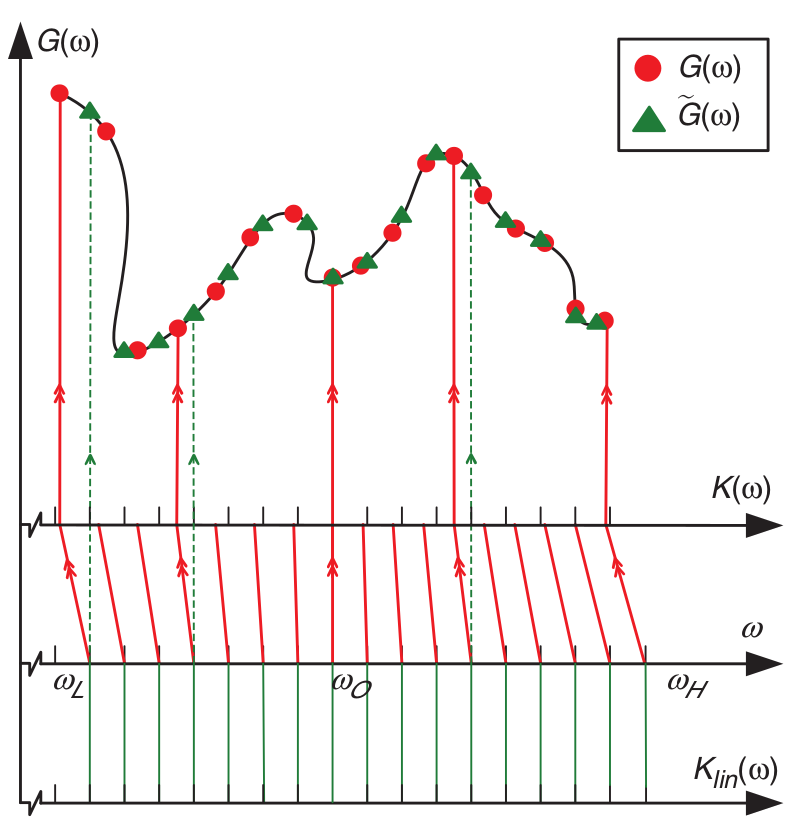
\includegraphics[width=13cm]{Zdjecia/4/algo_Taylora}
\caption{Wizualizacja algorytmu []Przypis do Pialucha}
\label{fig:algo_Taylora}
\end{figure}

Przedstawia on krzywą $G(\omega)$ z aż trzema osiami poziomymi. Linia ciągła przedstawia zależność $G(K(\omega))$, czerwonymi kółkami oznaczony jest sygnał $G(\omega)$. Jak widać przejście z dziedziny $K(\omega)$ na $\omega$ jest nieliniowe co wynika z niliniowego charakteru krzywej dyspersji. Zielonymi trójkątami oznaczono natomiast krzywą $G(K_{lin}(\omega))$. Jak widać przejście z dziedziny $\omega$ na $K_{lin}(\omega)$ jest przejściem o charakterze liniowym. 
\subsection{Wybrane wyniki symulacji}
Rysunek \ref{fig:liniakrzyws} obrazuje przybliżenie krzywej dyspersji wyznaczonej dla zadanego sygnału z rysunku 4.8.
\begin{figure}[h]
\centering
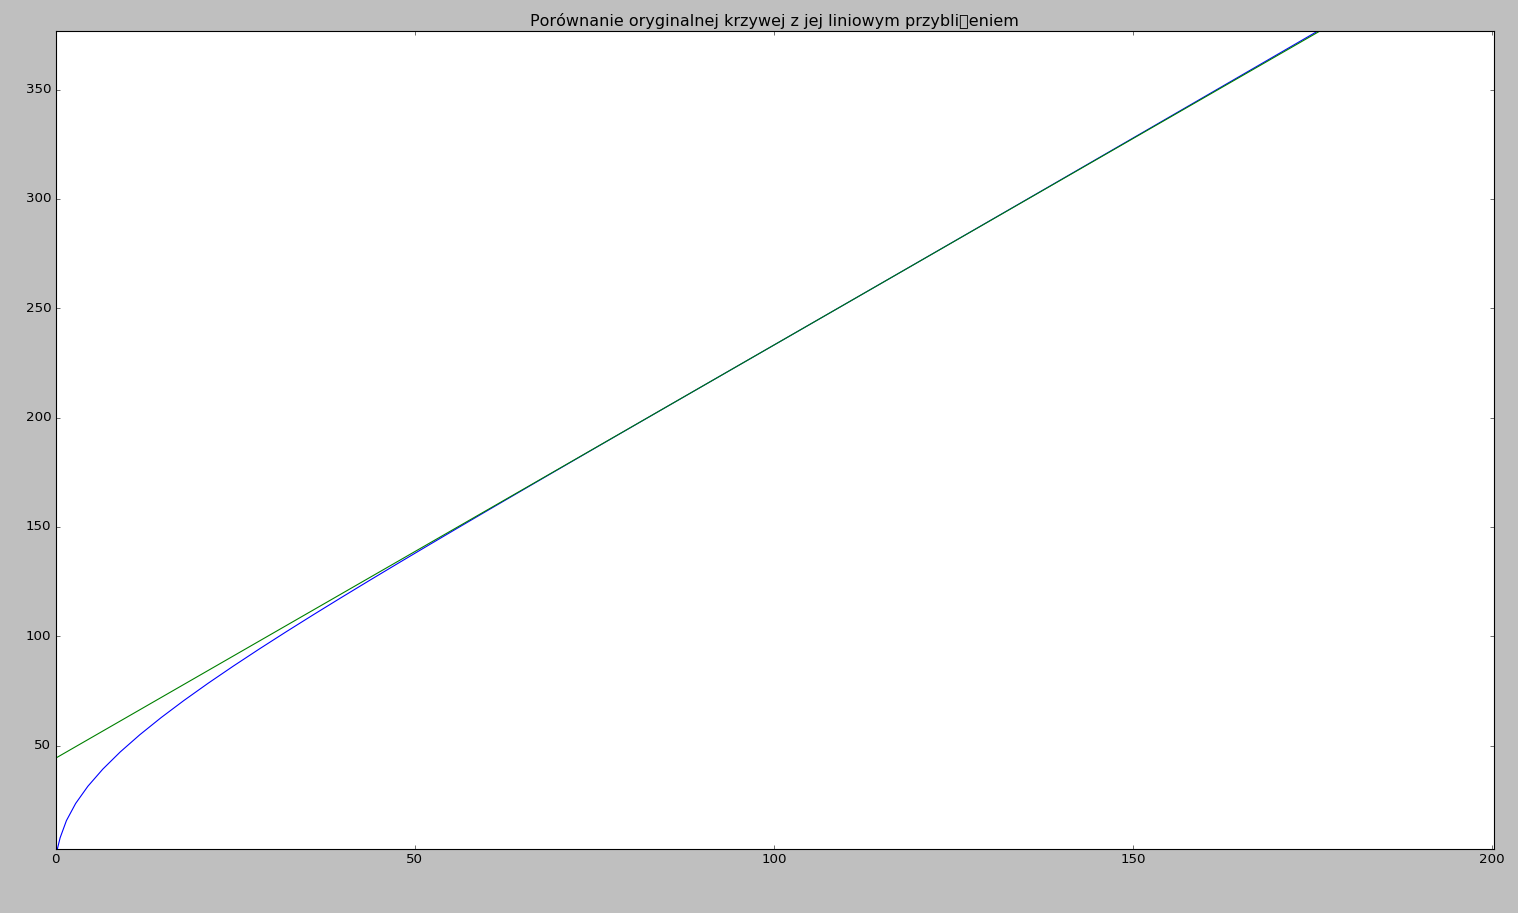
\includegraphics[width=13cm]{Zdjecia/4/krzywa_moja}
\caption{Porównanie oryginalnej krzwej z jej liniowym przybliżeniem}
\label{fig:liniakrzyws}
\end{figure}
Rysunek \ref{fig:przedipo} ilustruje przykład sygnału przed i po kompensacji.
\begin{figure}[h]
\centering
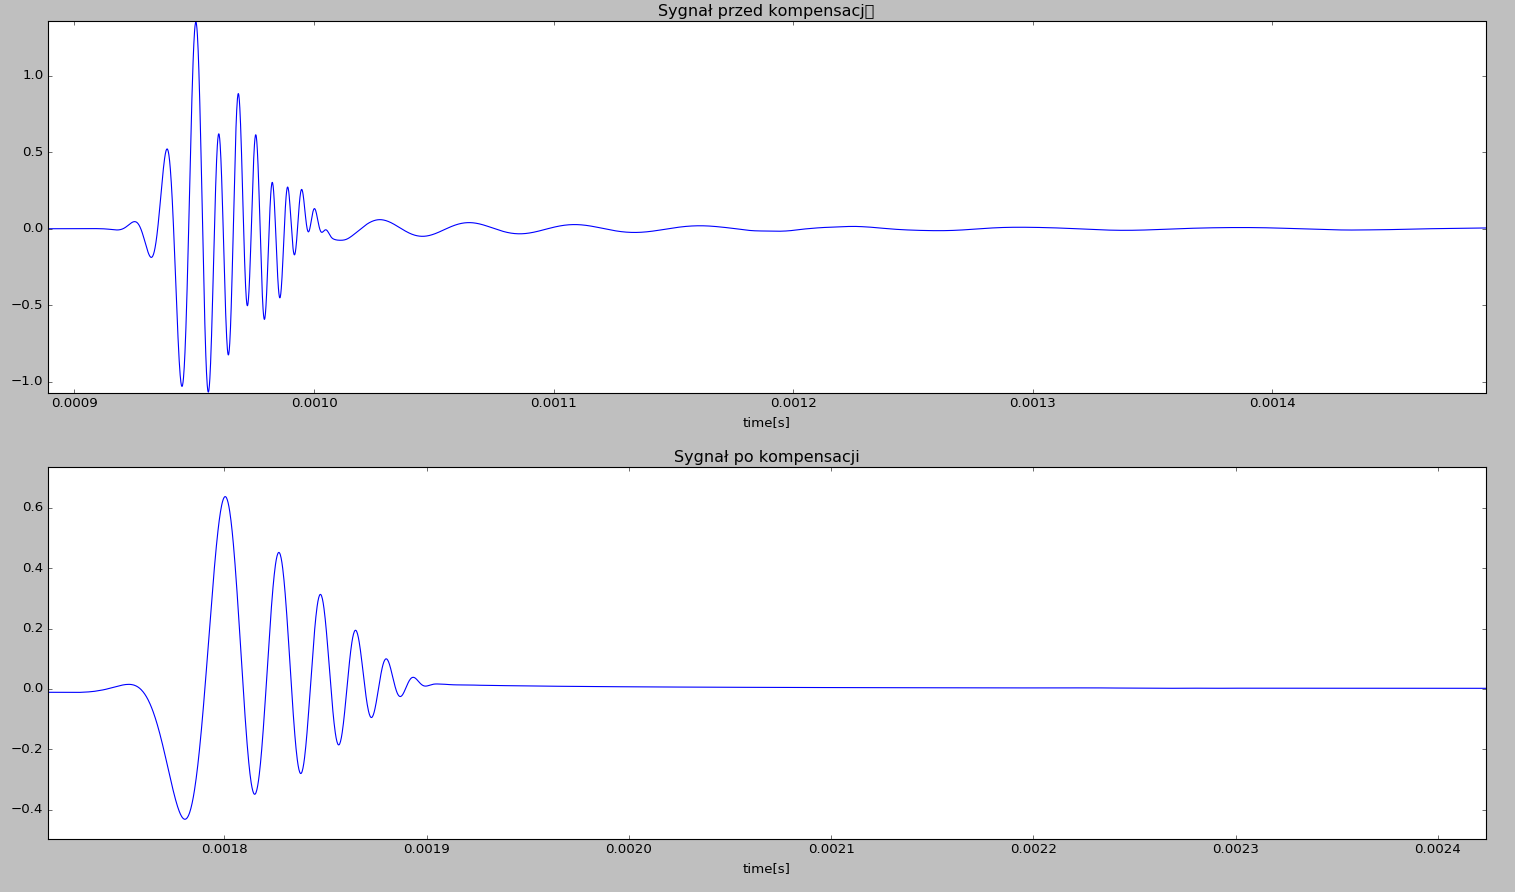
\includegraphics[width=13cm]{Zdjecia/4/przedipo}
\caption{Porównanie sygału przed i po kompensacji}
\label{fig:przedipo}
\end{figure}
Na ostatnim rysunku przedstawione zostało porównanie otrzymanych w wyniku kompensacji sygnałów z sygnałem zadanym \ref{fig:przedipo2}
\begin{figure}[h]
\centering
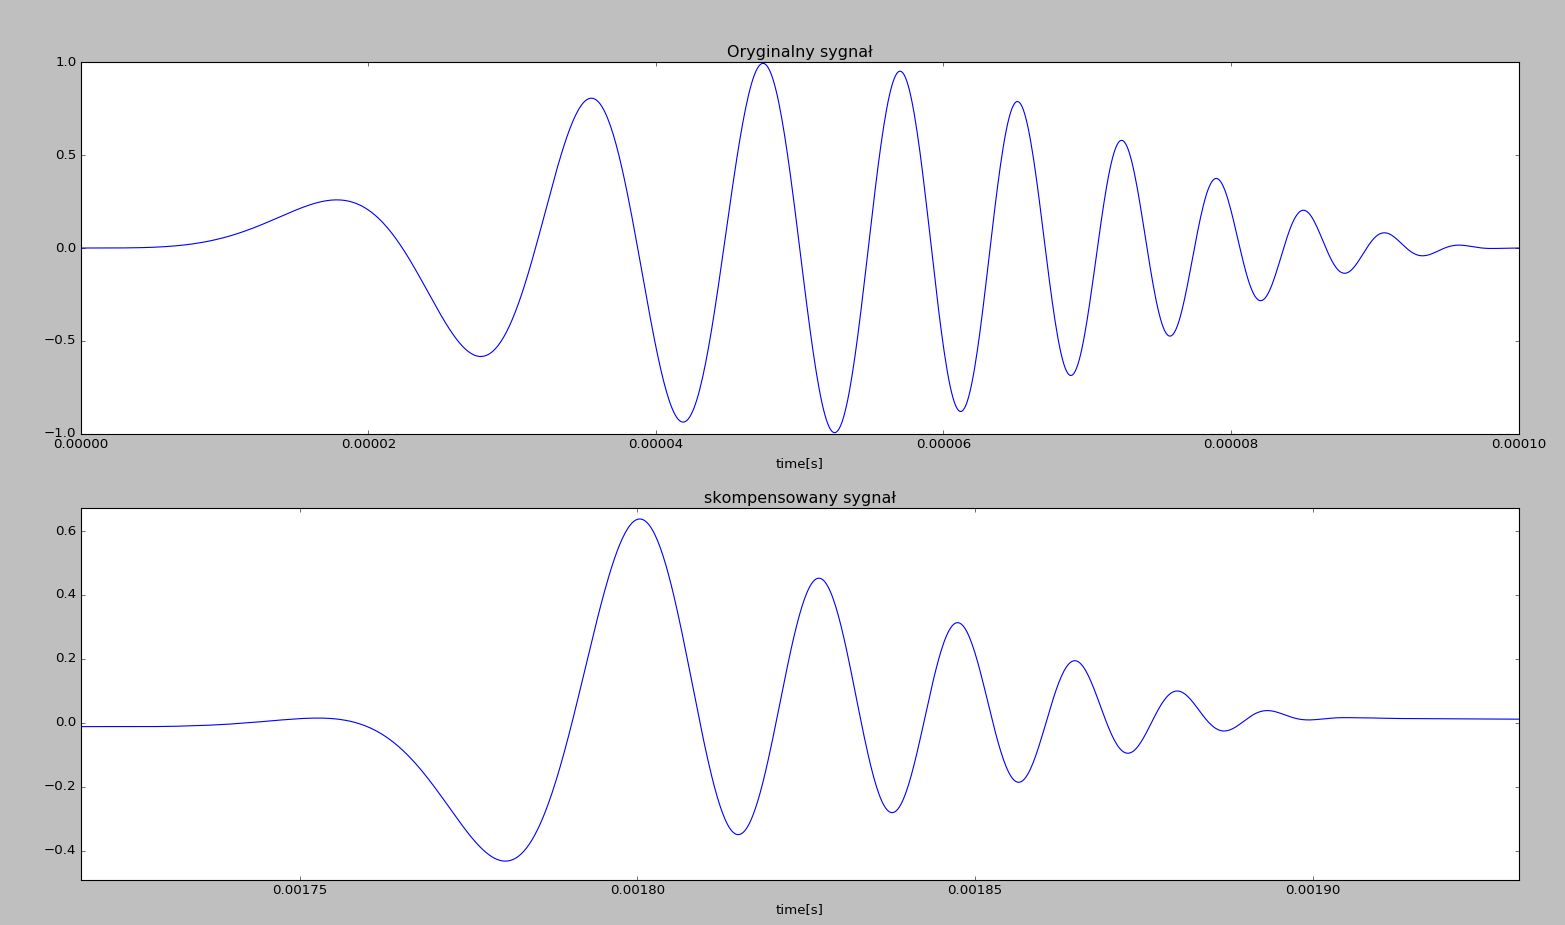
\includegraphics[width=13cm]{Zdjecia/4/przedipo2}
\caption{Porównanie sygnału oryginalnego z sygnałem skompensowanym}
\label{fig:przedipo2}
\end{figure}

\section{Metoda mapowania sygnału z dziedziny czasu na dziedzinę odległości}
\label{sec:Wilcox}

Opisana w poniższej sekcji metoda została zaprezentowana w artykule \cite{kasia1}. Opiera się na odpowiednim zastosowaniu transformaty Fouriera. Pozwala na kompensację sygnału poprzez przejście z dziedziny czasu na dziedzinę odległości, dzięki czemu w wyniku otrzymywany jest skompensowany sygnał oraz informacja o długości ścieżki propagacji.

\subsection{Podstawy teoretyczne}

W niniejszej pracy rozważaną strukturą, w której powstają i propagują fale prowadzone jest długi stalowy pret. Przyjmując oznaczenie sygnału wejściowego jako $f(t)$, natomiast propagujący w pręcie sygnał jako $u(x,t)$ zakłada się iż w miejscu wzbudzenia, zachodzi zależność: 
\begin{equation}
u(x,t) = f(t)
\end{equation}
Znając $u(x,t)$ w jednym punkcie w przestrzeni oraz znając charakterystykę propagującego trybu lub trybów fali prowadzonej, można odtworzyć sygnał po dowolnej odległości propagacji oraz w dowolnym punkcie czasowym. Można to osiągnąć rozważając przesunięcie fazowe każdej składowej częstotliwości oddzielnie:
\begin{equation}
u(x,t) = \int\limits_{-\infty}^{\infty}F(\omega)e^{i(k(\omega)x - \omega t)}d\omega \label{eq:propagacja_jeden_mod}
\end{equation}
Propagacja więcej niż jednego trybu fali oznacza, iż dana częstotliwość wzbudziła więcej niż jedną jej postać. Co za tym idzie w takim przypadku również możliwe jest odtworzenie przebiegu fali poprzez lekką modyfikację wzoru \ref{eq:propagacja_jeden_mod}
\begin{equation}
u(x,t) = \int\limits_{-\infty}^{\infty}F(\omega)e^{ -i \omega t}\sum \limits _{j=1}^{n}e^{ik_j(\omega)x} d\omega\label{eq:propagacja_kilka_mod}
\end{equation}
gdzie:

$F(\omega)$ - transforamta Fouriera sygnału $f(t)$

$k_j(omega)$ - wartość j-tej liczby falowej odpowiadającej częstotliwości $\omega$

Jak już zostało wspomniane, otrzymany sygnał g(t) można odwzorować na funkcję odległości bez stosowania algorytmu komepnsacji jedynie poprzez proste odwzorowanie:
\begin{equation}
x=v_{gr}t \label{eq:x=vgrt}
\end{equation}

Gdzie $v_{gr}$ jest prędkością grupową trybu fali prowadzonej, mierzoną zazwyczaj dla częstotliwości środkowej, lub tej o największej energii. Odwzorowanie takie jest proste do osiągnięcia poprzez zwykłe skalowanie osi czasu g(t) na odległośći propagacji. W przypadku takiego odwzorowania, możliwości wykrycia defektów struktury, znajdujących się w bliskiej odległości od innych cech strukturalnych takich jak na przykład koniec badanego pręta czy punkt łączenia dwóch prętów, zależy od czasu trwania poszczególnych sygnałów. Długie sygnały będą się na siebie nakładać co może doprowadzić do niewykrycia uszkodzenia. Z tego względu sygnał g(t) powinien być jak najkrótszy. 

Przedstawiany algorytm kompensacji dyspersji, zastępuje proste mapowacznie czasu na odległość przy pomocy równania \ref{eq:x=vgrt} takim, które jest wykonywane w domenie liczby falowej. Takie podejście pozwala wziąć pod uwagę prędkości zależne od częstotliwości, czyli wzięcie pod uwagę dyspersji. Niezbędnym elementem omawianej metody jest znajomość krzywych dyspresji badanego obiektu, w zakresie propagowanych trybów. Dokładność z jaką wyliczone krzywe reprezentują rzeczywistą charakterystykę układu, znajduje odzwierciedlenie w jakości uzyskanych wyników. W sytuacji idelanej przedstawiany algorytm przywraca każdy sygnał do dokładnego kształtu pierwotnego, niezależnie od jego odległości propagacji.  

Celem omawianej metody jest przekształcenie otrzymanego sygnału $g(t)$ w funkcję odległości propagacji a nie czasu, oraz skompensowanie rozproszenia otrzymanego sygnału. Dalsze propagowanie otrzymanego sygnału zarówno w przód jak i w tył można otrzymać stosując wzór \ref{eq:propagacja_jeden_mod} lub \ref{eq:propagacja_kilka_mod}. Gdyby obliczyć kompletną mapę odległościowo czasową, sygnał propagujący dalej rozpraszałby się coraz mocniej zarówno w czasie jak i przestrzeni. Natomiast sygnał propagujący wstecz zbiegłby się do swojego minimum w pewnym punkcie, a następnie ponownie rozproszył. Minimum jego trwania przypadłoby na chwilę czasową $t=0$. Dobrze ilustruje to rysunek \ref{fig:Wilcox_propaguje}
\begin{figure}[h]
\centering
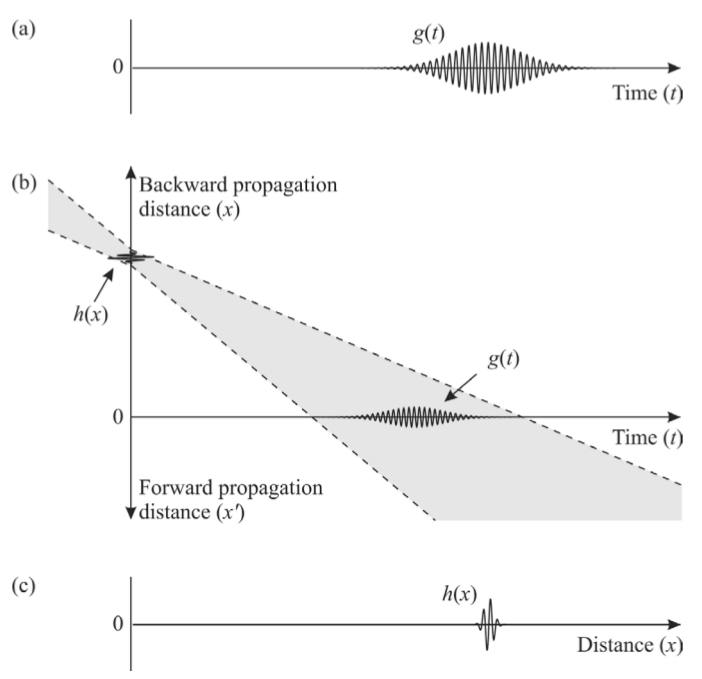
\includegraphics[width=14cm]{Zdjecia/4/Wilcox_zasada_dzial}
\caption{Zasada działania omawianej techniki kompensacji dyspersji \cite{kasia1}}
\label{fig:Wilcox_propaguje}
\end{figure}
Obliczenie propagowanego wstecz sygnału dla ujemnych wartości $x'$ w $t=0$ daje dokładnie poszukiwane odwzorowanie z czasu na odlgełość propagacji, która jest poszukiwana i która kompensuje rozproszenie odebranych sygnałów. Nowa zmienna propagacji $x'$ może być zdefiniowana jako $x=-x'$. Wynika z tego, iż propagacja wsteczna może zostać opisana wzorem:

\begin{equation}
h(x) = u(-x',0) = \int \limits_{-\infty}^{\infty}G(\omega)e^{-ik(\omega)x}d\omega \label{eq:wsteczna propagacja}
\end{equation}

gdzie:

$G(\omega)$ - transformata Fouriera odebranego sygnału w dziedzinie czasu $g(t)$

$h(x)$ - skompensowany dyspersyjnie przebieg odległości.

Funkja h(x) przedstawiona jest na rysunku \ref{fig:Wilcox_propaguje} (c).

W niniejszej pracy nie został uwzględniony współczynnik odbicia $A_j$. Na potrzeby symulacji przyjęte zostało iż jest on stały, niezależny od czestotliwości i wynosi 1. Gdyby jednak brać go pod uwagę to wzór 4.16 przyjałby postać:
\begin{equation}
g(t) = \sum \limits _{j}\int\limits_{-\infty}^{\infty}A_j(\omega)F(\omega)e^(ik(\omega)x_j-wt)d\omega
\end{equation}

W przyadku stałego współczynnika odbić wszystkie sygnały w h(x) powinny mieć ten sam kształt obwiedni co oryginalny sygnał wejściowy. Gdyby jednak zależał on od częstotliwości , wówczas obwiednia sygnału w h(x) zostanie zniekształcona i na ogół wydłużona. Takie zniekształcenie jest artefaktem charakterystycznym dla danego punktu odbicia fali. Co za tym idzie takie zakłócenie byłoby obserwowane nawet, gdyby zjawisko dyspersji nie występowało. 

\subsection{implementacja numeryczna}
Równanie \ref{eq:wsteczna propagacja} jest podstawowym równaniem omawianej metody. Jest równaniem kompensacji dyspersji dla funkcji ciągłych. W praktyce sygnał g(t) nie jest sygnałem ciągłym a sygnałem dyskretnym, wygenerowanym w aplikacji lub otrzymanym z przetwornika. Na potrzeby tego rozdziału przyjmijmy nastepujące oznaczenia:

$m$ - liczna próbek sygnału g(t)

$\Delta t$ - okres próbkowania sygnało g(t)

$m\Delta t$ - całkowity czas trwania sygnału g(t)

$n$ - liczba próbek otrzymanego sygnału w dziedzinie odległośći h(x)

$\Delta x$ -przestrzenny okres próbkowania h(x)

$n\Delta x$ - całkowita przestrzenna długość sygnału

Najprostszą implementacją omawianego algorytmu jest poddanie sygnału g(t) szybkiej transformacie Fouriera, a następnie całkowanie numeryczne w zakresie częstotliwości sygnału wejściowego. Takie rozwiązanie byłoby niezwykle czasochłonne ponieważ całkowanie musiałoby zostać wykonane dla każdego z n punkót w skompensowanym sygnale h(x). Metodą, która została zaimplementowana w opisanej aplikacji polega na modyfikacji równania \ref{eq:wsteczna propagacja}. Ta zmiana pozwala na wykonywanie całkowania w ramach algorytmu odwrotnej transformaty Fouriera. Skompensowany sygnał jest funkcją odległości. Odwrotna transformata Fouriera musi zostać zastosowana na sygnale w dziedzinie liczby falowej. Wynika z tego, iż zmienna całkowania w równaniu \ref{eq:wsteczna propagacja} musi zostać zmieniona z $\omega$ na $k$. Można to łatwo zrobić używając poniższych zależności:
\begin{equation}
d\omega = v_{gr}(\omega)dk
\end{equation}
\begin{equation}
\omega = v_{ph}(\omega)k
\end{equation}

Gdzie:

$v_{gr}(\omega)$ - prędkość grupowa propagującej postaci

$v_{ph}(\omega)$ - prędkość fazowa propagującej postaci

Biorąc to pod uwagę równanie \ref{eq:wsteczna propagacja} można zapisać jako:


\begin{equation}
h(x) = \int\limits_{-\infty}^{infty}H(k)e^{-ikx}dk \label{eq:h(x) dobre}
\end{equation}

\begin{equation}
H(k) = G(k)v_gr(k)
\end{equation}

$$
\omega = \omega(k)
$$

Równanie \ref{eq:h(x) dobre} ma postać odwrotnej transformaty Fouriera $H(k)$, w punktach spróbkowanych ze stałym przestrzennym okresem próbkowania $\Delta k$. Uzyskana z transformaty Fouriera funkcja $G(\omega)$ jest funkcją o punktach równomiernie spróbkowanych w dziedzinie częstotliwości. Ze względu na nieliniowy charakter krzywych dyspersji przejście z dziedziny częstości na dziedzinę liczby falowej dałoby w rezultacie funkcję o nierównomiernie spróbkowanej osi k. Aby uzyskać porządany efekt konieczne jest użycie znanej z krzywej dyspersji zależności między wartościami $\omega$ oraz $k$, aby interpolować funkcję G, tak by znaleźć jej wartości w punktach równomiernie rozmieszczonych w dziedzinie liczby falowej.

$G(\omega)$ jest sygnałem zawierającym informacje zarówno o fazie jak i amplitudzie sygnału. W rozwiązaniu numerycznym istotne jest aby dobrać odpowiednie wartości kroków. Zbyt duże ich wartości mogą spowodować utratę informacji, natomiast zbyt małe prowadzą do znacznego wydłużania czasu obliczeń, w zamian za co uzyskiwane wyniki są dokładniejsze i wpływ szumu staje się mniej znaczący. W celu zmniejszenia szumu powodowanego przez błędy interpolacji w końcowym, skompensowanym sygnale, otrzymany sygnał g(t) wypełnia się zerami.W aplikacji użytkownik ma możliwość samodzielnie podać ile razy chce wydłużyć sygnał poprzez wypełnienie zerami. Ograniczenim podlega zarówno $\Delta k$ jak i ilość punktów liczb falowych n. Aby zapobiec zawijaniu sygnału w domenie odległości, minimalna długość skompensowanego sygnału h(x) musi być większa od długości pierwotnego sygnału g(t) pomnożonego przez maksymalną prędkość grupową $v_{max}$.
\begin{equation}
n\Delta x > m\Delta tv_{max}\label{eq:nierownosc dlugosci sygnalow}
\end{equation} 

Powyższa nierówność określa nam maksymalny rozmiar kroku liczby falowej jako:

\begin{equation}
\Delta k = \frac{1}{n\Delta x} < \frac{1}{ m\Delta tv_{max}}\label{eq:nierown delta k}
\end{equation}

Aby cała energia pierwotnego sygnału została poprawnie odwzorowana na dziedzinę odległości, liczba falowa Nyquista $k_{Nyq}$ musi być większa lub równa liczbie falowej trybu fali prowadzonej o częstotliwości Nyquista $f_{Nyq}$ oryginalnego sygnału. Co można zapisać jako:
\begin{equation}
k_{Nyq}\geq k(f_{Nyq})\label{eq:k Nyquista}
\end{equation}
$$
\geq k(\frac{1}{2\Delta t})
$$

Nierówność \ref{eq:k Nyquista} oraz równanie \ref{eq:nierown delta k} pozwalają określić minimalną liczbę punktów w sygnale h(x)
\begin{equation}
n > 2\frac{k_{Nyq}}{\Delta k}
\end{equation}

W zaimplementowanym algorytmie, pierwszym krokiem jest wydłużenie otrzymanego sygnału zadaną ilość razy oraz wykonanie szybkiej transformaty Fouriera na wydłużonym sygnale. Następnie na podstawie przedstawionych ograniczeń dobierana jest wartość kroku $\Delta k$ oraz obliczana wartość $k_{max} = k(\omega _{max})$. Znając te parametry tworzony jest wektor zawierający równomiernie rozłożone wartości liczby falowej. Przy użyciu krzywej dyspersji, interpolując liniowo potrzebne wartości obliczana jest funkcja $G(k)$ oraz $v_{gr}(k)$ w tych samych punktach. Następnie wyliczana zostaje funkcja $H(k)$ mająca równomiernie rozłożone wartości liczby falowej. Ostatnim etapem jest zastosowanie szybkiej odwrotnej transformaty Fouriera co pozwala uzyskać poszukiwany sygnał h(x).

W przypadku gdy mamy do czynienia z propagacją większej ilości postaci fal lub gdy podczas odbicia następuje konwersja trybu fali prowadzonej dokonywane jest uśrednianie propagowanych postaci. Przy założeniu, że propagują jednocześnie dwie postacie równanie \ref{eq:wsteczna propagacja} można ponownie zapisać jako:
\begin{equation}
h(x) = \int\limits _{-\infty}^{\infty}G(\omega)e^{i(k_1(\omega)+k_2(\omega))\frac{x}{2}}d\omega \label{eq:wiele postaci}
\end{equation}
W implementacji oznacza to, iż kilka krzywych dyspersji zostaje ośrednionych do jednej postaci w której $k_{12} = \frac{1}{2}(k_1(\omega) + k_2(\omega))$
\subsection{Wybrane wyniki symulacji}
Przykładowe sygnał wejściowy wygenerowane w aplikacji zaprezentowane zostały na rysunku \ref{fig:przykl_we}.
\begin{figure}[h]
\centering
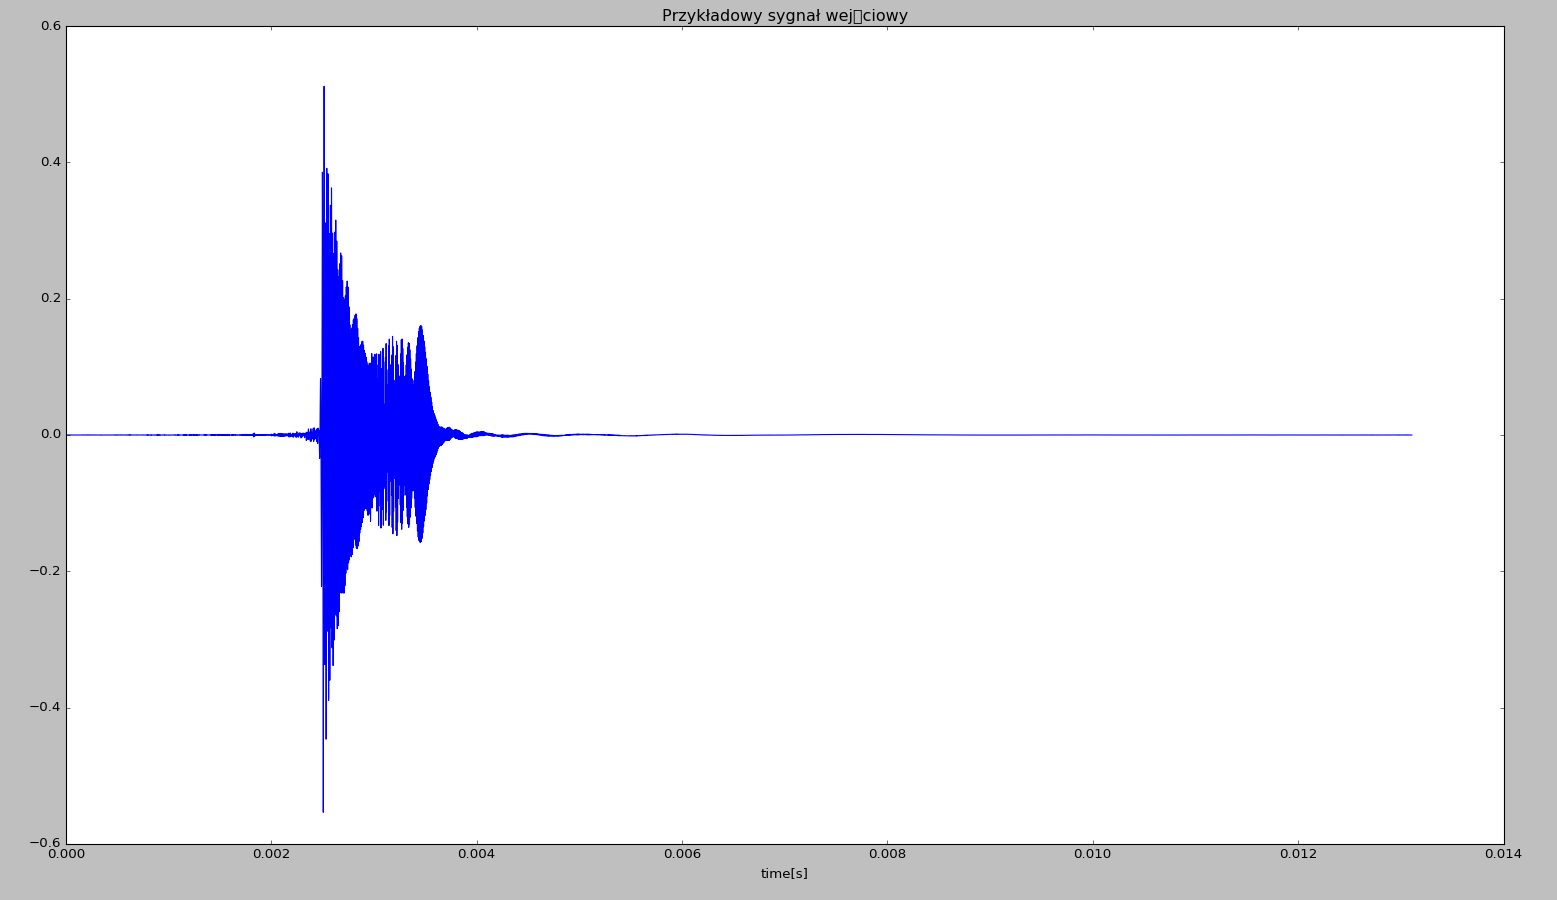
\includegraphics[width=14cm]{Zdjecia/4/przykl_we}
\caption{przykładowy sygnał wejściowy}
\label{fig:przykl_we}
\end{figure}
Przykładowa krzywa dyspersji powstała w wyniku uśrednienia trzech pierwszych postaci fali zaprezentowana została na rysunku \ref{fig:mean}. 
\begin{figure}[h]
\centering
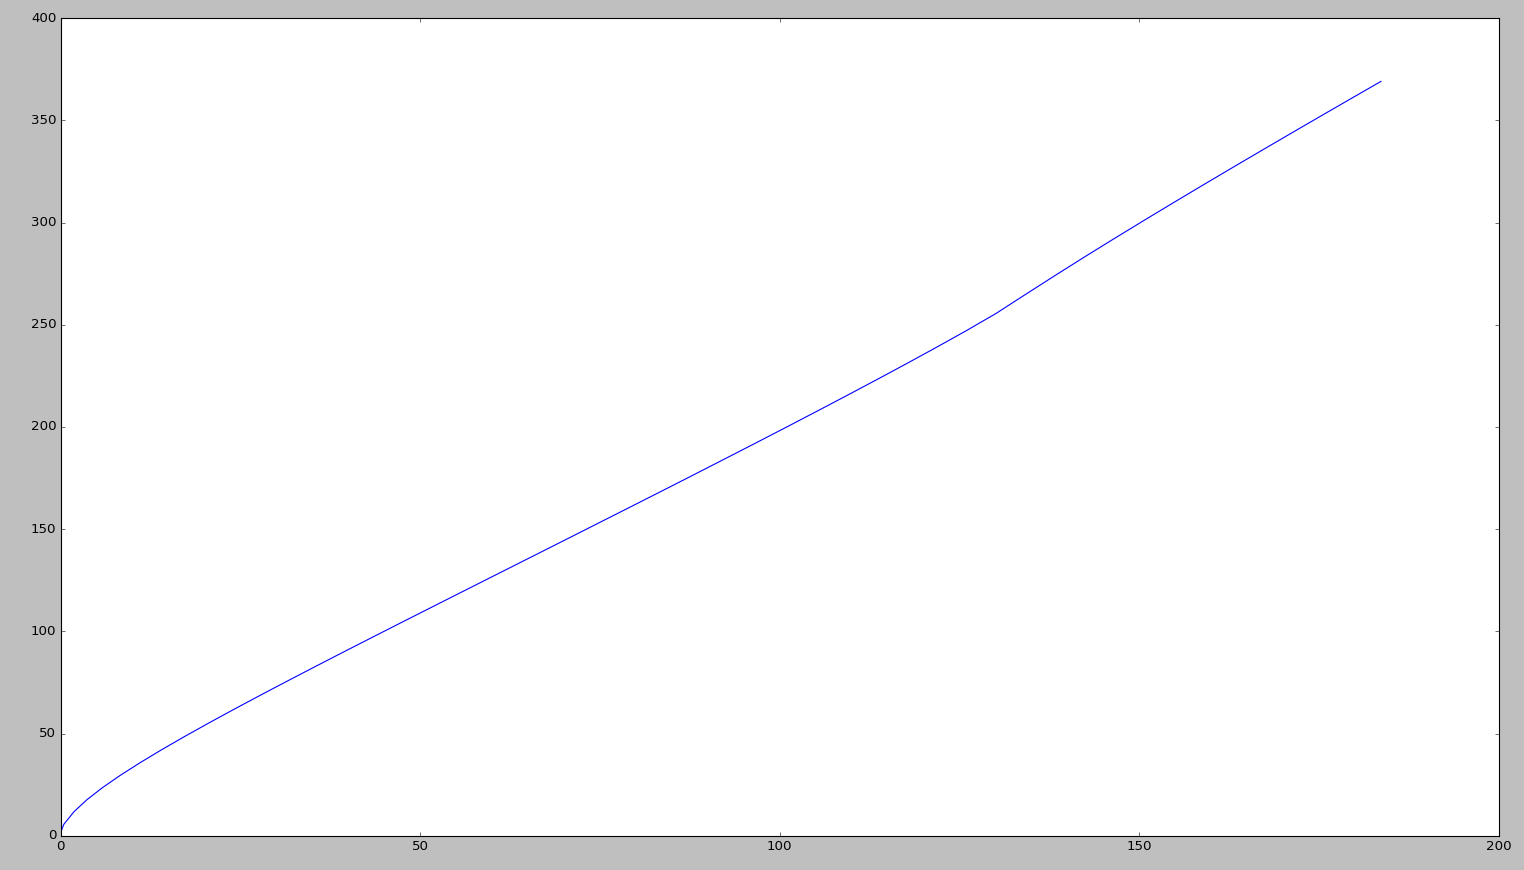
\includegraphics[width=14cm]{Zdjecia/4/meanmode}
\caption{Średnia krzywa dyspersji powstała z uśrednienia trzech pierwszych krzywych}
\label{fig:mean}
\end{figure}
Na kolejnym rysunku \ref{fig:wil1} przedstawiono porównanie sygnału przed i po kompensacji. Rozproszony sygnał został skompensowany do znacznie krótszej postaci. Dodatkowo w łatwy sposób możliwe jest odczytanie długości ścieżki propagacji, która w tym przypadku wynosiła dwa metry. 
\begin{figure}[h]
\centering
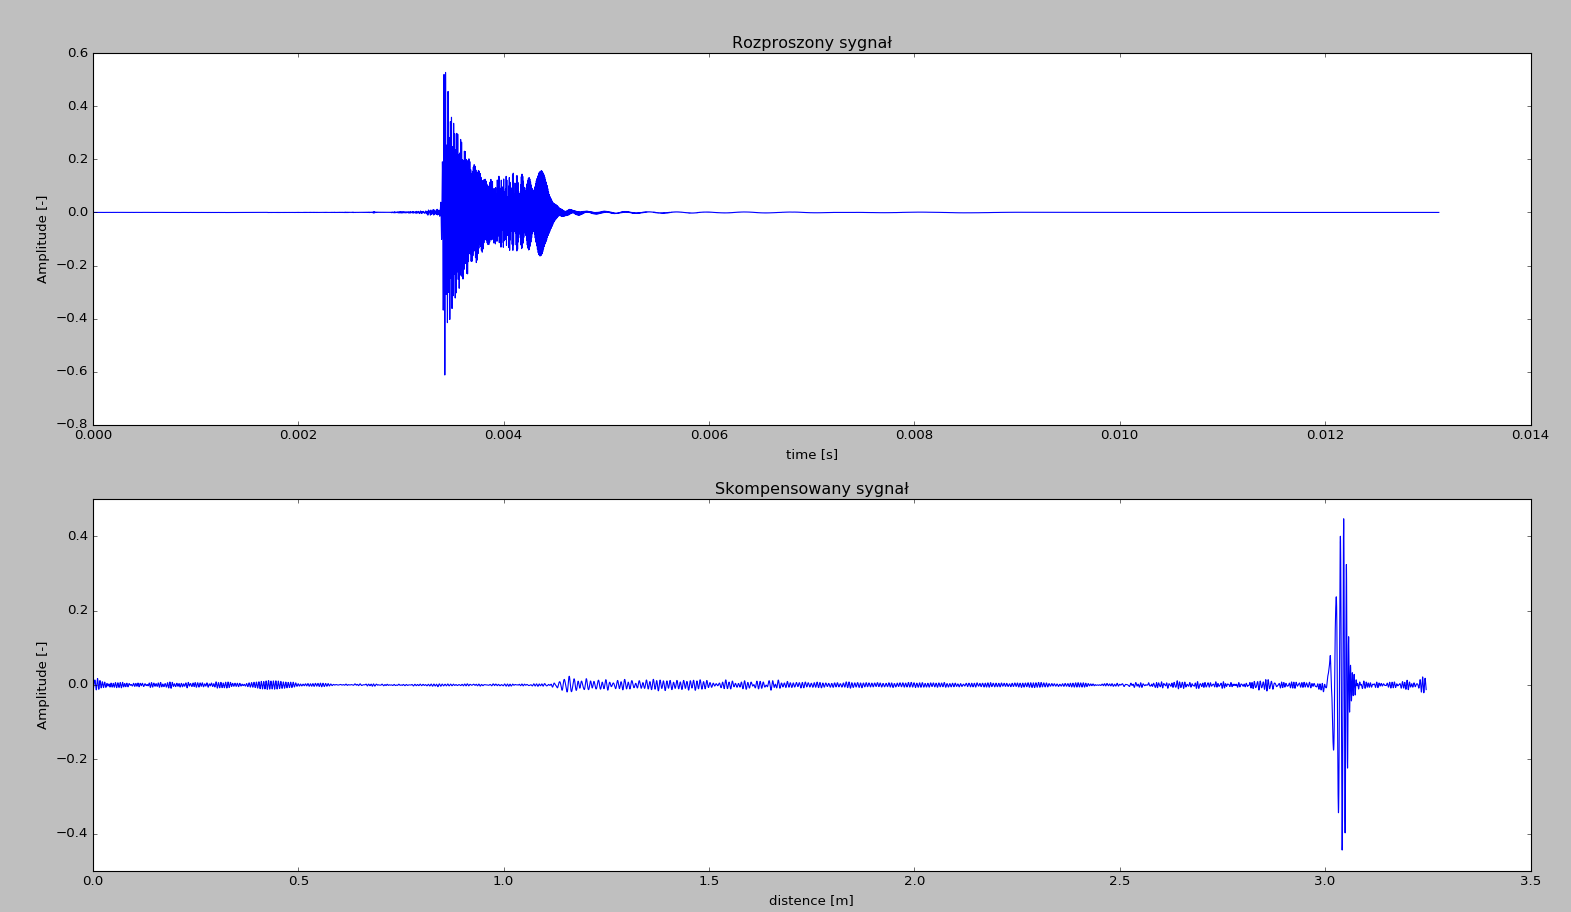
\includegraphics[width=14cm]{Zdjecia/4/wilcox1}
\caption{Porównanie sygnału przed i po kompensacji}
\label{fig:wil1}
\end{figure}
Kolejny rysunek przedstawia wyniki symulacji, w której sygnał nie został dostatecznie wydłużony w wyniku czego otrzymany wynik był nieczytelny \ref{fig:zawij}
\begin{figure}[h]
\centering
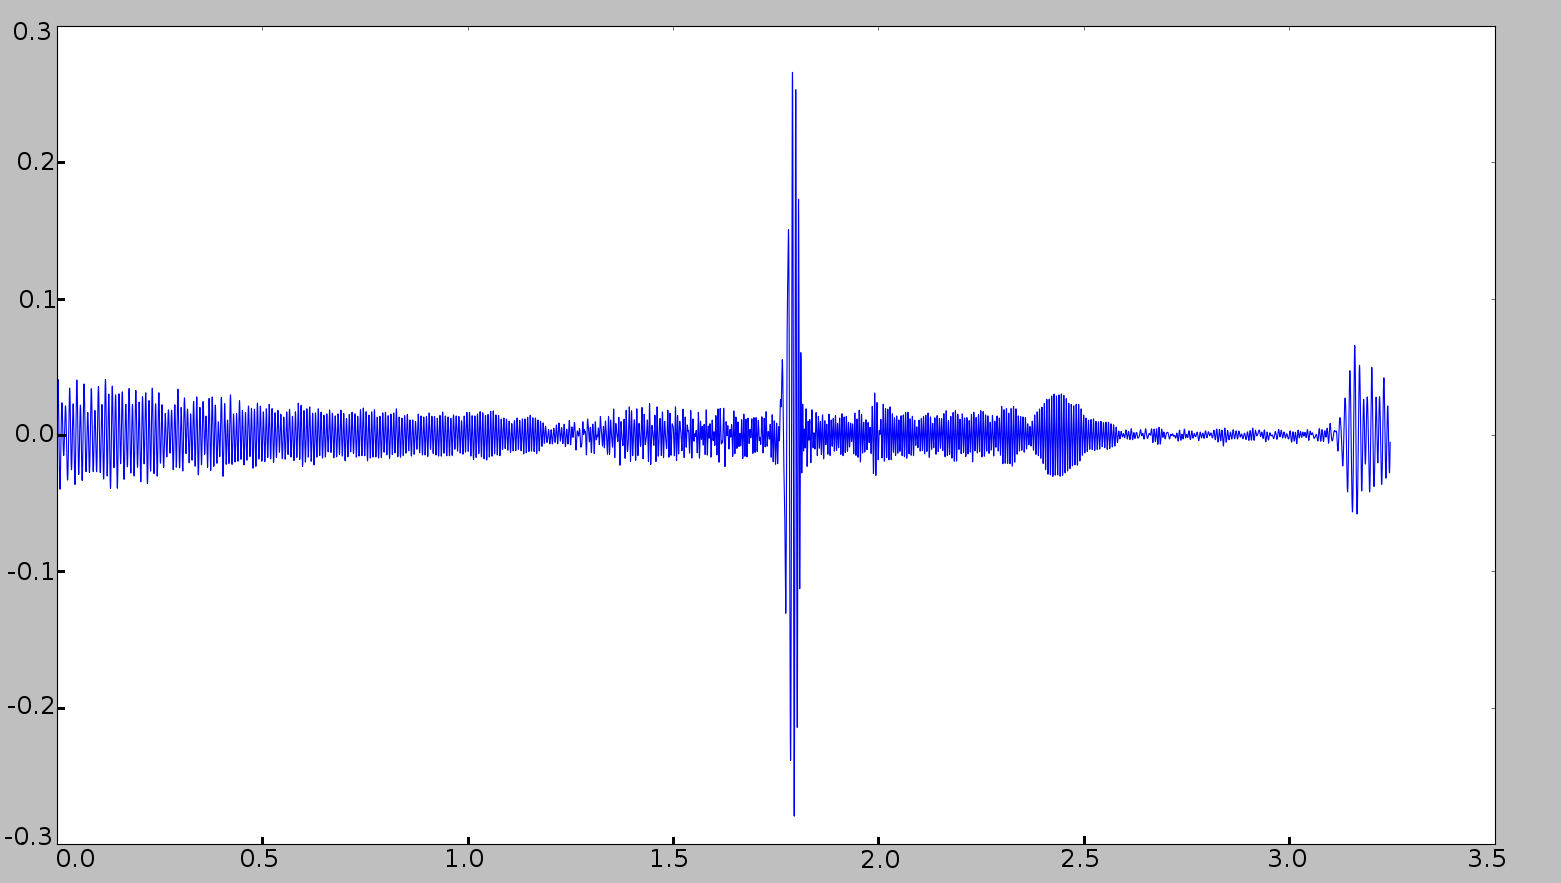
\includegraphics[width=14cm]{Zdjecia/4/naklada}
\caption{Sygnał, który przepropagował 5 metrów, widoczne zawijanie sygnału}
\label{fig:zawij}
\end{figure}
Ostatni rysunek prezentuje porównanie skompensowanego sygnału z sygnałem wejściowym, w przypadku, gdy symulowana była propagacja pierwszych trzech postaci fali prowadzonej. Omawiana metoda daje najlepsze wyniki kompensacji. Ze wszystkich prezentowanych w ramach niniejszej pracy metod, ta najdokładniej odwzorowuje zadany na wejściu sygnał. Jej kolejnymi atutami są minimalne wymagania jeśli chodzi o dane wejściowe oraz największa ilość otrzymywanych informacji. Na podstawie znajomości jedynie przepropagowanego sygnału oraz znajomości krzywych dyspersji propagujących postaci jest ona w stanie skompensować rozproszony sygnał, podając jednocześnie informację o długości ścieżki propagacji. Algorytm radzi sobie dobrze zarówno z kompensacją jednej propagującej postaci jak i dwiema a nawet trzema.

\begin{figure}[h]
\centering
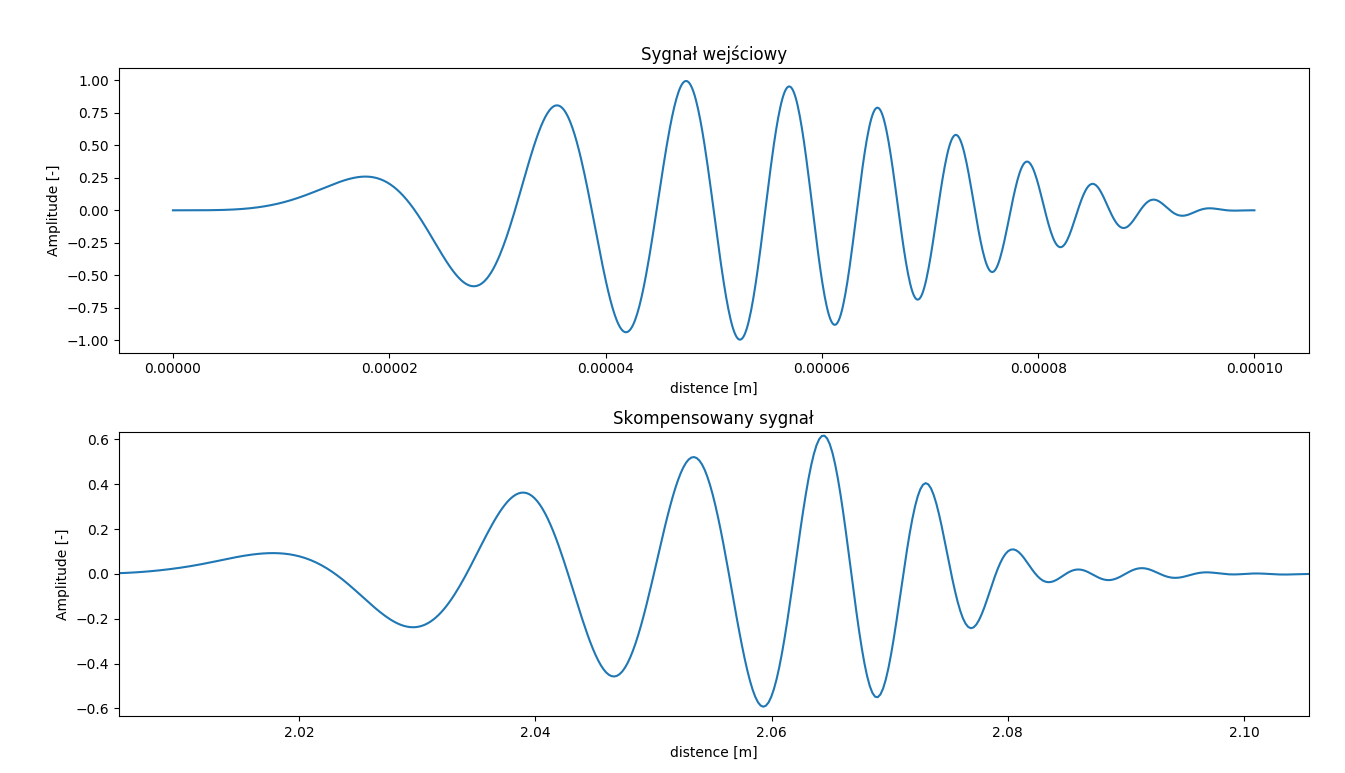
\includegraphics[width=14cm]{Zdjecia/4/Wilcoxporownanie}
\caption{Porównanie sygnału wejściowego oraz sygnału skompensowanego}
\label{fig:willast}
\end{figure}

\subsection{Przykład zastosowania na podstawie symulacji wybranego pręta}

Na potrzeby symulacji, jako testowany obiekt, przyjęty został pręt wykonany ze stali czarnej o grubości 25 mm długości dwóch metrów. Stałe materiałowe wyniosły odpowiednio: 

współczynnik Poissona - $\nu$ = 0.3 

moduł Younga - E = 210 GPa 

Pierwszym etapem było wygenerowanie odpowiednich krzywych dyspersji. Zostały one przedstawione na rysunku \ref{fig:krzywestalowe}
\begin{figure}[h]
\centering
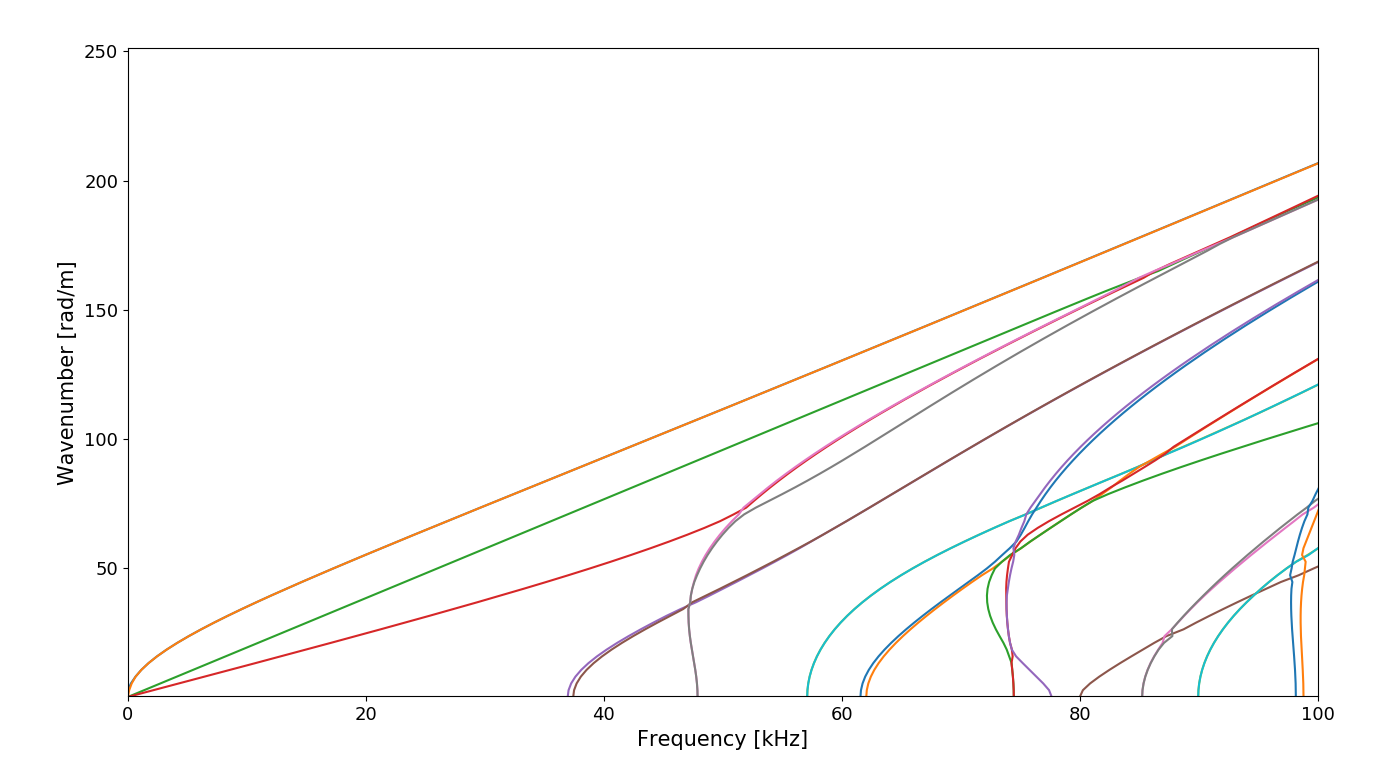
\includegraphics[width=14cm]{Zdjecia/4/krzywestalowe}
\caption{Krzywe dyspersji analizowanego pręta}
\label{fig:krzywestalowe}
\end{figure}

Do ich wygenerowania użyte zostały czworościenne elementy skończone. Płaszczyzna złożona z ośmiu okręgów, w pierwszym z nich wygenerowane osiem punktów. Rozkład punktów na pojedynczej płaszczyźnie przedstawia wysunek \ref{fig:punktynaplaszczyznie}

\begin{figure}[h]
\centering
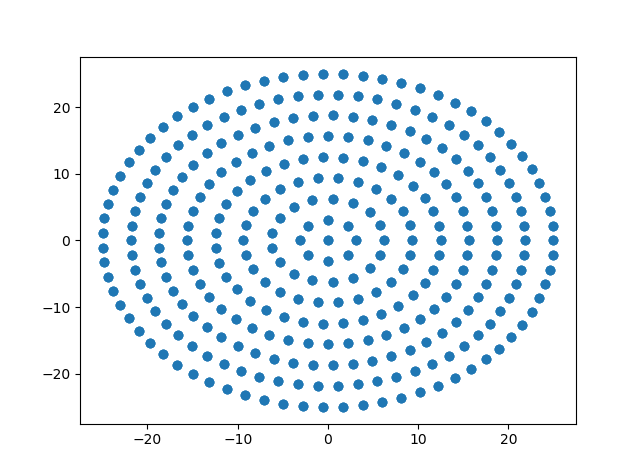
\includegraphics[width=14cm]{Zdjecia/4/siatka}
\caption{rozkład punktów modelu MES na płaszczyźnie, użyty do generacji modelu}
\label{fig:punktynaplaszczyznie}
\end{figure}

Do symulacji użyty został sygnał linear chirp, opisany na początku tego rozdziału. Pierwszym krokiem jest jego odpowiednie wydłużenie w czasie poprzez dołożenie na jego końcu odpowiedniej ilości zer. Następnie wykonana została symulacja propagacji tak przygotowanego sygnału na dystans dwóch metrów. Symulacja taka odpowiada sytuacji, w której odpowiedni wzbudnik zostałby umieszczony na jednym z końców badanego obiektu, natomiast na jego drugim końcu znalazłby się odpowiedni odbiornik. Do symulacji przyjęte zostało, iż w badanym obiekcie propagują trzy pierwsze postaci fali prowadzonej. Wyniki symulacji przedstawione zostały na rysunku \ref{fig:sygnalrozproszony}

\begin{figure}[h]
\centering
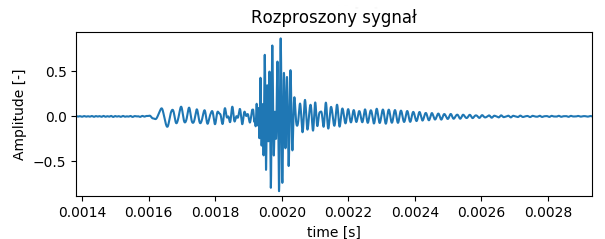
\includegraphics[width=14cm]{Zdjecia/4/sygnalrozproszony}
\caption{Sygnał rozproszony, uzyskany drogą symulacji}
\label{fig:sygnalrozproszony}
\end{figure}

Kolejnym krokiem jest kompensacja tak otrzymanego sygnału. Otrzymany drogą symulacji, rozproszony sygnał został przekazany do funkcji kompensującej. W wyniku kompensacji otrzymany zostaje sygnał zmapowany na dziedzinę odległości. Z otrzymanych wyników łatwo odczytać, iż długość ścieżki propagacji wyniosła dwa metry. Jest to dokładnie taka odległość na jaką sygnał wejściowy został przepropagowany zaraz na początku. Uzyskany omawianą metodą sygnał przedstawiony został na rysunku \ref{fig:skompensowanysygnal}.

\begin{figure}[h]
\centering
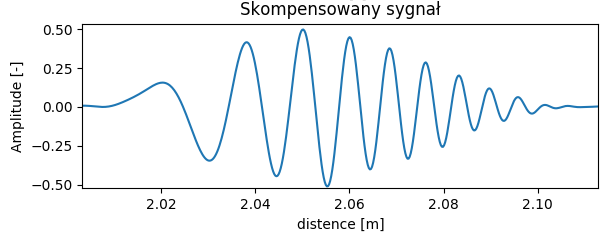
\includegraphics[width=14cm]{Zdjecia/4/sygnalskompensowany}
\caption{Sygnał skompensowany omawiana metodą}
\label{fig:skompensowanysygnal}
\end{figure}

Ostatnie rysunek przedstawia zestawienie pozwalające na porównanie: sygnału wejściowego, sygnału rozproszonego oraz sygnału skompensowanego. łatwo zauważyć, iż sygnał przed kompensacją uległ dyspersji i jest znacznie rozproszony, co uniemożliwiłoby jego identyfikacje oraz określenie, czy badana struktura nie jest uszkodzona. Sygnał po kompensacji, jest niemal identyczny z sygnałem zadanym. 

\begin{figure}[h]
\centering
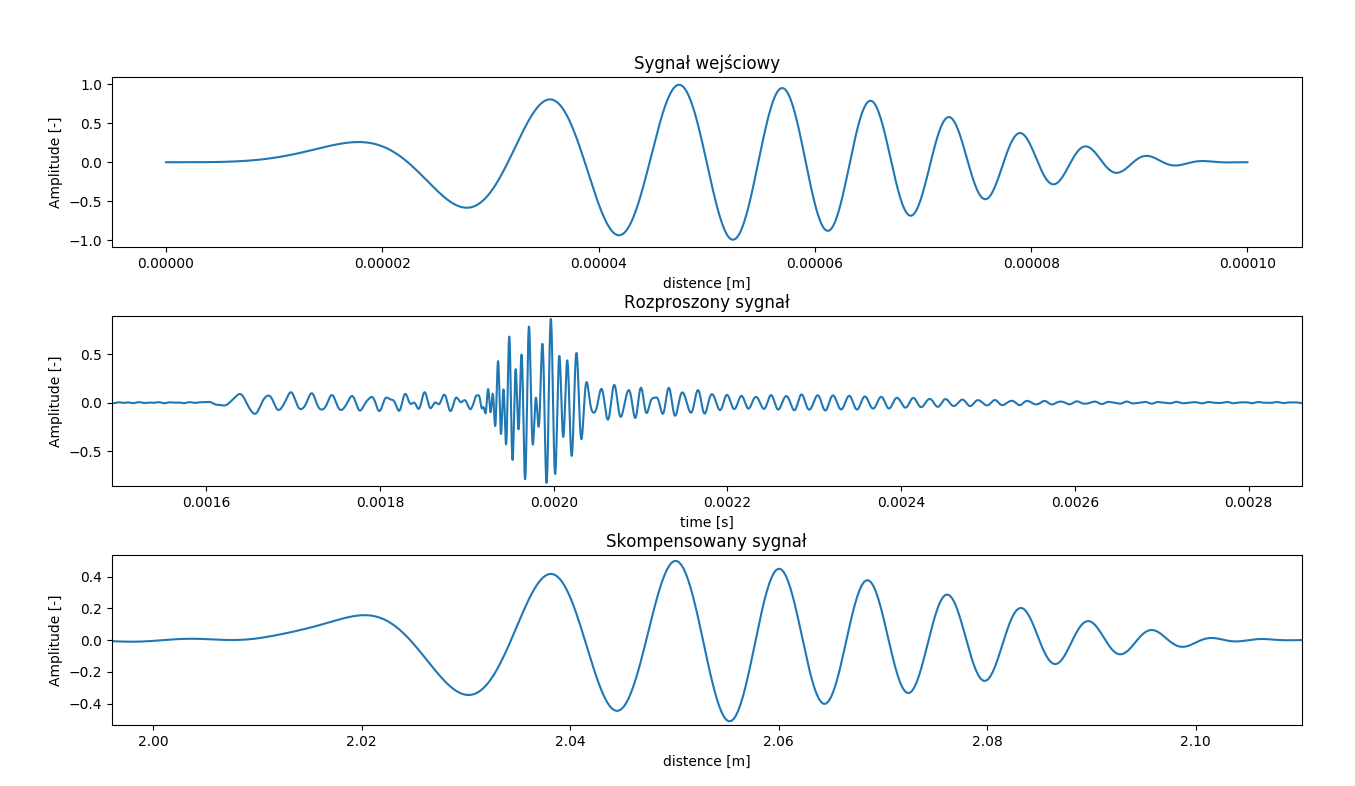
\includegraphics[width=14cm]{Zdjecia/4/porownaniewszystkichsygnalow}
\caption{Porównanie sygnałów: wejściowego, rozproszonego oraz skompensowanego}
\label{fig:porownaniewszystkich}
\end{figure}

Stworzona aplikacja pozwala zatem na kompleksową symulację fali prowadzonej w zadanym pręcie. Znając parametry fizyczne zadanego materiału, możliwe jest wygenerowanie modelu pręta wykonanego z dowolnego materiału, oraz dowolnej długości. Możliwa jest również symulacja propagacji fali prowadzonej na dowolną odległość oraz, co zostało opisane w tym rozdziale, kompensacja dyspersji trzema wybranymi metodami. Jak widać na powyższym przykładzie omawiana metoda pozwala na uzyskanie bardzo dobrych wyników symulacyjnych.
\section{Porownanie opracowanych metod kompensacji}

W tym rozdziale opisane zostały wybrane trzy metody kompensacji dyspersji, które zostały zainplementowane do stworzonej aplikacji w ramach niniejszej pracy. Każda z przedstawionych metod ma zarówno wady jak i zalety i ograniczenia. W poniższym podrozdziale znajduje się porównanie opracowanych metod.
\subsection{Metoda odwracania sygnału w czasie}
Zalety:
\begin{enumerate}
\item Szybkość działania - ze wszystkich zaimplementowanych metod ta pozwala w najkrótszym czasie uzyskać rządane rezultaty.
\item Skuteczność kompensacji - sygnał otrzymany w wyniku symulacji kompensuje się do postaci sygnału wejściowego z dokładnością do kolejności w czasie
\item Możliwość kompensacji sygnału wielopostaciowego - Metoda ta ze względu na swoją prostotę pozwala na skompensowanie zarówno sygnału będącego rozproszonym pojedynczym trybem fali prowadzonej jak i sygnału będącego złożeniem kilku rozproszonych postaci tej fali 
\end{enumerate}

Wady i ograniczenia:
\begin{enumerate}
\item Znana długość ścieżki propagacji - aby wygenerować żądany sygnał musi być znana długość ściażki propagacji, po przebyciu której sygnał powinien się skompensować.
\item Otrzymany sygnał odwrócony w czasie - otrzymany po propagacji sygnał nie jest identyczny z żądanym sygnałem. Jak pokazano w symulacji otrzymany sygnał jest żądanym sygnałem odwróconym w czasie
\item Trudności w zastosowaniu w przypadku więcej niż jednego punktu odbicia - w przypadku odbić od kilku powierzchni, jak na przykład w przypadku badanie dwóch połączonych ze sobą prętów, stworzenie sygnału, który wprowadzony do obiektu powróci w skompensowanej formie jest trudniejsze i wymagałoby wielu prób heurystycznych.
\item Konieczność znajomości krzywych dyspersji - Aby móc wygenerować odpowiedni sygnał, który skompensuje sie na zadanej odległości, niezbędna jest znajomość krzywych dyspersji do wstępnej symulacji sygnał.
\end{enumerate}
Podsumowując, największą zaletą tej metody jest jej szybkość działania. Pomimo ograniczenia w postaci konieczności posiadania informacji o długości ścieżki propagacji, metoda ta wydaje się być skuteczna do kontroli zbadanych wcześniej obiektów. W przypadku badań heurystycznych wydaje się iż jej dodatkowym atutem może być brak konieczność znajomości krzywych dyspersji. Być może wystarczyłoby wcześniej zbadać obiekt, czyli wprowadzić do obiektu sygnał, który ostatenie chcemy otrzymywać po propagacji. Otrzymany eksperymentalnie sygnał odwrócić w czasie i znów wprowadzić do pręta. Tak przygotowany sygnał również powinien skompensować się podobnie jak w symulacji, jednak z pewnością już po pierwszej propagacji, w sygnale pojawią się szumy, które ostatecznie mogą pogarszać otrzymywane wyniki. Metoda wydaje się być dobra do kontroli dobrze, zbadanych obiektów, co do których należy się tylko upewnić, że nie powstały żadne uszkodzenia od czasu ostatniej kontroli. W takim wypadku po zadaniu sygnału oczekiwany jest konkretny rezultat, w przypadku pojawienia się uszkodzeń, które spowodują dodatkowe i przedwczesne odbicie sygnału, otrzymany sygnał świadczyć będzie o uszkodzeniu. Nie dostarczy nam jednak informacji o miejscu jego wystąpienia.

\subsection{Metoda mapowania liniowego przy pomocy rozwinięcia w szereg Taylora}
Zalety:
\begin{enumerate}
\item Kompensacja dowolnej ilości odbić zadanego sygnału - Przedstawiona metoda pozwala na kompensację dowolnej ilości odbić sygnału wejściowego. Jeśli tylko punkty odbić nie będą zbyt blisko siebie, sygnały po kompensacji da się rozróżnić i określić liczbę punktów odbicia
\item Możliwość oszacowania długości ścieżki propagacji - znając prędkość grupową częstotliwości o najwyższej energii oraz czas przybycia sygnału możliwe jest oszacowanie długość ścieżki jego propagacji.
\end{enumerate}
Wady i ograniczenia:
\begin{enumerate}
\item Czas obliczeń - ze wszystkich zaimplementowanych metod czas obliczeń tej jest najdłuższy.
\item Niedokładne odwzorowanie sygnału wejściowego - Wyniki z symulacji pokazują, iż ta metoda pomimo, że kompensuje sygnał do postaci zbliżonej do tej wejściowej to jednak jego obwiednia wydaje się być nieco zniekształcona w stosunku do oryginału
\item Możliwość kompensacji tylko pojedyńczej postaci fali - przedstawiona metoda pozwala na skompensowanie dyspersji tylko w przypadku, gdy mamy do czynienia z pojedyńczym trybem fali.
\item Znana krzywa dyspersji propagującego trybu fali - jest to informacja niezbędna do skompensowania sygnału.
\end{enumerate}
Podsumowując, prezentowana metoda pozwala na skompensowanie sygnału odbitego od dowolnej ilości punktów. Jednak jej zasadniczym ograniczeniem jest propagacja fali tylko w jednej postaci, co jednak jest możliwe do osiągnięcia dzięki odpowiednio dobranemu wzbudnikowi oraz wyliczeniu postaci, która ma zostać wzbudzona oraz tych które powinny być stłumione. Przy odpowiednio spreparowanym sygnale wejściowym, zapewniającym propagację jedynie wybranej postaci fali, metoda ta powinna skutecznie skompensować dyspersję oraz pozwolić na oszacowanie odległości na jakich znajdują się punkty odbicia, co za tym idzie zlokalizować potencjalne uszkodzenia.
\subsection{Metoda mapowania sygnału z dziedziny czasu na dziedzinę odległości}
Zalety:
\begin{enumerate}
\item Otrzymywana informacja o długości ścieżki propagacji - metoda ta przynosi podwójne korzyści, poniewąż oprócz skompensowanego sygnału dostarczana jest automatycznie również informacja o długości ścieżki propagacji sygnału. Otrzyman sygnał wyjściowy jest sygnałem w dziedzinie odległości, więc długość ścieżki propagacji można odczytać bezpośrednio z wygenerowanego wyniku
\item Kompensacja dowolnej ilości propagujących postaci oraz dowolnej liczby odbić sygnału - Jedynym elementem wymaganym aby skompensować otrzymany sygnał jest znajomość krzywych dyspersji opisujących propagujące postaci. Metoda pozwala na skompensowanie sygnału zarówno jednomowego jak i takiego, który zawiera kilka postaci fali.
\item szybkość działania - mimo iż zaimplementowany algorytm działa nieco dłużej niż pierwsza z omawianych metod, ta również dokonuje obliczeń w dość zadawalającym czasie. Dodatkowym atutej jest to, ze poprzez drobne zmiany w aplikacji jesteśmy w stanie sterować szybkością jej działania. Poprzez zmianę odpowiednich parametrów użytkownik jest w stanie zdecydować czy zależy mu na dokładności wyników czy na szybkości wykonywanego algorytmu.
\item Jakość wyników - wyniki uzyskane z symulacji pokazują, iż kompensacja tą metodą pozwala na dokładne odwzorowanie sygnału wejściowego. Im dokładniejsze są opisujące go krzywe dyspersji tym otrzymany w wyniku kompensacji sygnał lepiej odwzorowuje stan faktyczny.
\end{enumerate}
Wady i ograniczenia:
\begin{enumerate}
\item znajomość krzywych dyspersji - tak jak i poprzednie metody tak i ta również wymaga znajomości funkcji opisujących badany obiekt. Potrzebna jest również informacja o tym, które postaci zostały wzbudzone i propagowały w badanym obiekcie.
\end{enumerate}
Ta metoda jest najskuteczniejszą z opracowanych w ramach tej pracy metod. Posiada najmniej ograniczeń jednocześnie pozwalając uzyskać najdokładniejsze rezultaty. Długość ścieżki propagacji nie tylko nie musi być znana jak również jest bezpośrednio przekazywana użytkownikowi wraz ze skompensowanym sygnałem.
